%!Tex Program = xelatex
%\documentclass[a4paper]{article}
\documentclass[a4paper]{ctexart}
\usepackage{xltxtra}
%\setmainfont[Mapping=tex-text]{AR PL UMing CN:style=Light}
%\setmainfont[Mapping=tex-text]{AR PL UKai CN:style=Book}
%\setmainfont[Mapping=tex-text]{WenQuanYi Zen Hei:style=Regular}
%\setmainfont[Mapping=tex-text]{WenQuanYi Zen Hei Sharp:style=Regular}
%\setmainfont[Mapping=tex-text]{AR PL KaitiM GB:style=Regular} 
%\setmainfont[Mapping=tex-text]{AR PL SungtiL GB:style=Regular} 
%\setmainfont[Mapping=tex-text]{WenQuanYi Zen Hei Mono:style=Regular} 

\usepackage{listings}
\usepackage{xcolor}
\usepackage{amsmath}
\usepackage{amsthm}
\usepackage{amssymb}
\usepackage{mathrsfs}
\usepackage{enumitem}  
\usepackage{tikz}
\usepackage{booktabs}

\definecolor{codegreen}{rgb}{0,0.6,0}
\definecolor{codegray}{rgb}{0.5,0.5,0.5}
\definecolor{codepurple}{rgb}{0.58,0,0.82}
\definecolor{backcolour}{rgb}{0.95,0.95,0.92}

\lstdefinestyle{mystyle}{
    backgroundcolor=\color{backcolour},   
    commentstyle=\color{codegreen},
    keywordstyle=\color{magenta},
    numberstyle=\tiny\color{codegray},
    stringstyle=\color{codepurple},
    basicstyle=\ttfamily\footnotesize,
    breakatwhitespace=false,         
    breaklines=true,                 
    captionpos=b,                    
    keepspaces=true,                 
    numbers=left,                    
    numbersep=5pt,                  
    showspaces=false,                
    showstringspaces=false,
    showtabs=false,                  
    tabsize=2
}

\lstset{style=mystyle}

%\newfontfamily\yuanti{cwTeXYen} 

% 创建一个特定的定理样式和计数器  
\newtheorem{theorem}{定理}  
%\newtheorem{example}{例}
\newtheorem{remark}{备注}  

\newtheorem{definition}[theorem]{定义} % 定义 'definition' 环境    
% 创建其他定理样式并使用上述“theorem”的计数器  
\newtheorem{lemma}[theorem]{引理}  
\newtheorem{corollary}[theorem]{推论}  
\newtheorem{proposition}[theorem]{命题}  
%\newtheorem*{proposition}{命题}  
\newtheorem*{theorem*}{定理}  
\newtheorem{example}[theorem]{例}
\newtheorem{note}[theorem]{注记}
\newtheorem{challenge}[theorem]{挑战}  
\newtheorem{exercise}[theorem]{练习}  
\newtheorem{algorithm}[theorem]{算法}  

\numberwithin{theorem}{section}  
\numberwithin{equation}{section} 
\numberwithin{figure}{section} 
\numberwithin{remark}{section} 


\title{数值分析}
\author{王何宇}
\date{}

\begin{document}
\maketitle
\pagestyle{empty}

这里大部分同学不是第一次见到我, 或者是第一次上我的课了. 所以很多事情可
以简要一点.

\begin{itemize}
\item 王何宇, 手机: 13456940632,
\item Email: wangheyu@zju.edu.cn
\item 办公室: 海纳苑2幢,1208, 办公时间除了上课开会一般在, 但如果要来答疑最
  好先约一下.
\end{itemize}

这门课是信息与计算科学专业的必修课. 主要内容是科学计算的基础, 我们将默
认大家已经掌握了基本的分析学和代数学, 以及具备计算机操作和编程能力. 我
们将使用 C++ 来实现我们的算法. 这里强调一下, 从数值分析角度, 也许我们
并不一定要掌握 C++, 但掌握 C++ 的好处就是让大家能够深入算法和数据结构实现的底层.
同时为未来从事工业级别的编程的可能性留下基础.

这门课之后还有一门后续课程, 微分方程数值解. 在那门课上大家将真正掌握如
何用计算机对科学和工程问题进行模拟. 这里我强调: 我们绝不培养程序员. 我们培养的是有扎
实数学功底, 能操作复杂计算设备, 进行工业级别设计和编程能力的应用数学科
研工作者.

以下内容将不会出现在课堂讲授, 但会直接使用:
\begin{itemize}
%\item 基于 Linux 环境下的编程;
\item 数学分析、高等代数和概率论相关内容;
\item C++ 面向对象编程;
\item 基于 Latex 的科技文档编写;
\item 基于 git 的代码管理;
\end{itemize}

如果你缺乏上述能力, 大概率你并不是信息与计算专业同学, 或者强基班同学.
请慎重考虑一下是否真的要选修这门课. 如果你决定继续, 那么上述内容你必须
尽快自学. 课程群和助教会提供必要的学习资料.  

我们这门课在期末会有一个闭卷的理论考试, 非常符合我们数学院一致的风格.
将会是 8 道需要一定数学分析和代数技巧的证明题或计算题. 它将占总成绩的
60\%.

我们基本上除开学和期末以外, 每周都会布置一次作业, 总共大约有 10 余次作
业. 保留得分最高的 10 次, 作为你的平时作业成绩. 平时作业成绩占总成绩的
25 \%. 注意, 作业允许延迟一周补交, 但分数打 8 折. 超过一周不再接受补交.

我们在期中会布置一次项目作业, 直到接近期末再交, 这个项目作业会有一定的
代码编程量和较为严格的文档规范. 项目作业占总成绩的 15\%. 项目作业的 DL
接近期末, 因此不接受补交. 

以上三块成绩合成即为你的最终成绩. 大家知道, 一般在考试当晚 12 点, 我会
上传你的最终成绩. 所以请放心, 我不会给大家留下求分时间.

最后, 我们会不定期出现一些选做作业, 往往难度较高, 但给分较宽, 或者不存
在标准答案. 选做作业可以计入作业总数. 一个永恒的选做作业是指出我上课实
际性错误和讲义的任何错误(包括印刷错). 每指出一个错误根据严重程度会有
0.5 到 2 分的额外加分. 额外加分直接加在平时成绩总分上(总分 40 分计),
如果平时成绩已经加满, 按溢出分数多少给予适当物质奖励. 本课程同学如果在
钉钉答疑群解答同学技术问题, 助教会记录, 期末给予一定物质奖励.

强调一下我们学校, 学院, 系和我本人, 对学术诚信极为重视, 任何学术不端行
为都不能接受. 在本课堂, 学术不端行为包括:

\begin{itemize}
\item 考试作弊;
\item 作业抄袭;
\item 项目作业抄袭;
\end{itemize}

抄袭除了直接的文本和代码复制, 也包括剽窃他人思想或成果, 
且没有声明或引用. 这些行为除可能承担学校的纪律处分之外, 
作业抄袭首次出现将判为零分, 再次出现将判整个作业模块零分, 
并提请学院教学委员会取消其参加课程期末考试资格.

项目作业抄袭或学术剽窃则项目作业模块零分, 并视作一次作业抄袭行为.

如果你作业或者项目作业有困难, 助教和我都乐于提供帮助. 你也可以寻求同学
帮助, 但要在作业或项目作业中给予必要的声明, 并独立完成你的作业. 这些声
明本身不会影响对你的成绩判定.

对抄袭的判定主要由助教从作业客观表现提出, 并由教师判定. 必要的时候, 可
以邀请部分同学参与判定. %不论是教师还是助教, 对作业抄袭行为不接受举报. 

关于 AI,我们鼓励使用 AI 来提升学习效率,包括作业讨论。但要求在掌握之后能独立解决问题。
为此,我们要求:
\begin{itemize}
  \item 作业和项目作业中,必须声明使用了哪些 AI 工具。
  \item 作业和项目作业必须是独立完成的,不能直接复制 AI 的输出。如果作业留有 AI 痕迹(由助教判断),则会扣分;
  \item 如果发现作业或项目作业直接由 AI 生成,甚至未经任何修改。那么视作抄袭,处理方式等同抄袭;
  \item 如果你不同意助教的判定,提交 AI 对话记录时,可以申诉。
\end{itemize}

最后, 作为我个人的一个基本原则, 我遵守以下教学原则:

\begin{itemize}
  \item 我从不点名. 我鼓励学生根据自己的实际情况对学习的进度和方式作出
    调整. 但作为任课教师的多年经验, 客观上发现来教室听课的同学比不来教室听课的同学成绩有断崖式领先。
  \item 我不接受未毕业学生及一切相关利益人除拍马屁以外的任何利益输送,
    包括请吃饭. 概无例外. 鲜花和贺卡也不建议个人赠送.  
\end{itemize}

时间有限, 我们赶紧上车出发, 未尽事宜, 群里商量.

%% 我们会看到, 对用户而言, 算法可以就是一个黑盒. 用户可以既不懂其数学理论,
%% 也不懂如何编程实现, 比如游戏开发人员, 只要套用算法工具就行了. 或者比如
%% 数学家或者软件工程师, 他们能掌握算法的一面. 但是大家既然选择了信息与计
%% 算这个专业, 那就意味着你们必须以一种优雅的方式, 同时掌握算法的两面. 在
%% 这条道路上, C++ 是正确的选择. 同时这种技能会使你具备成为一个工业级别软
%% 件设计和开发者的潜力. 大家可能听说过, 码农干到35岁就会退休或上天台. 我
%% 2014年去英国访问时, 见到了我的博士导师的博士导师. 他已经从数学教授位置
%% 上退休了, 并且不再做数学研究. 但是他和他的两位同事, 都是70多岁的人, 一
%% 起写开发和编写工业软件, 并且招收了将近200个博士生之类的人作为助手. 大
%% 部分时间, 他们都可以一边喝茶一边吹牛, 只需在几个关键的点给出必要的指导
%% 就行了.


\section{求解非线性方程}

\begin{remark}
我们在中学时学会了解方程 $ax^2 + bx + c = 0$. 在更一般的情形中,方程 $f(x) = 0$ 的解析解可能并不存在。
因此我们需要研究如何\textbf{数值地}求解它。一个实际的例子是开普勒方程:
\[
x - a \sin x - b = 0,
\]
其中 $a$ 和 $b$ 的取值范围很大。这里 $a$ 是 $0 \sim 1$ 之间的数, 物理意义是偏心率, 
当 $a = 0$ 时, 行星轨道就是一个圆, 而越接近 $1$, 则轨道越是一个扁椭圆; 而 $b$ 是平均近点角(Mean Anomaly), 
是一个 $0 \sim 2 \pi$ 之间的数($b = 0$ 是近地点,$b = \pi$ 是远地点). 尽管这是一个很简单的方程, 
但也无法给出一个解析的求根公式. 
考虑一下如何数值求解该方程? (暴力一把?) 先画出来? 这也许是最朴素的求根算法.    
\end{remark}

\subsection{二分法}

\begin{algorithm}
    % alg 1.1
    \label{alg::bisection}
对于连续函数 $f : \mathbb{R} \to \mathbb{R}$ 的求根问题,\textbf{二分法} 通过不断将包含根的区间对半划分,并返回该区间中点作为解的近似值;参见图~\ref{fig::bisection}。
\end{algorithm}


\begin{remark}
为什么我们需要 $M, \delta, \epsilon$?答:这些都是为了实际的停止准则。$M$ 是最大迭代次数,
用于限制 CPU 时间开销;当 $M = 0$ 时表示不进行迭代。$\delta$ 与 $\epsilon$ 来源于计算机的有限精度。    

所以有限精度、有限时间是我们必须考虑的实际问题,也是和数学分析本质区别所在。
\end{remark}

\begin{figure}
\centering
\begin{minipage}{0.75\textwidth}
\textbf{输入:} $f : [a,b] \rightarrow \mathbb{R}$, $a \in \mathbb{R}, b \in \mathbb{R}$, \\
$M \in \mathbb{N}, \delta \in \mathbb{R}^+, \epsilon \in \mathbb{R}^+$ \\
\textbf{前提条件:} $f \in C([a,b])$, $\text{sgn}(f(a)) \neq \text{sgn}(f(b))$ \\
\textbf{输出:} $c, h, k$ \\
\textbf{后置条件:} $|f(c)| < \epsilon$ 或 $|h| < \delta$ 或 $k = M$

\begin{enumerate}
\item $u \leftarrow f(a)$
\item $v \leftarrow f(b)$
\item \textbf{for} $k = 0$ \textbf{to} $M$ \textbf{do}
\item \quad $h \leftarrow b - a$
\item \quad $c \leftarrow a + h/2$
\item \quad \textbf{if} $|h| < \delta$ 或 $k = M$ \textbf{then break}
\item \quad $w \leftarrow f(c)$
\item \quad \textbf{if} $|w| < \epsilon$ \textbf{then break}
\item \quad \textbf{else if} $\text{sgn}(w) \neq \text{sgn}(u)$ \textbf{then}
\item \qquad $b \leftarrow c$
\item \qquad $v \leftarrow w$
\item \quad \textbf{else}
\item \qquad $a \leftarrow c$
\item \qquad $u \leftarrow w$
\item \textbf{end for}
\end{enumerate}
\caption{二分法算法}
\label{fig::bisection}
\end{minipage}
\end{figure}

\subsection{算法的签名}

\begin{definition}
一个\textbf{算法}是一个逐步过程,它接受一组\textbf{输入}并生成一组\textbf{输出}。    
\end{definition}

\begin{definition}
一个\textbf{前提条件}是指对于执行算法,输入必须满足的条件。    
\end{definition}

\begin{definition}
一个\textbf{后置条件}是指在算法执行完成后,输出必须满足的条件。
\end{definition}

\begin{figure}
\centering
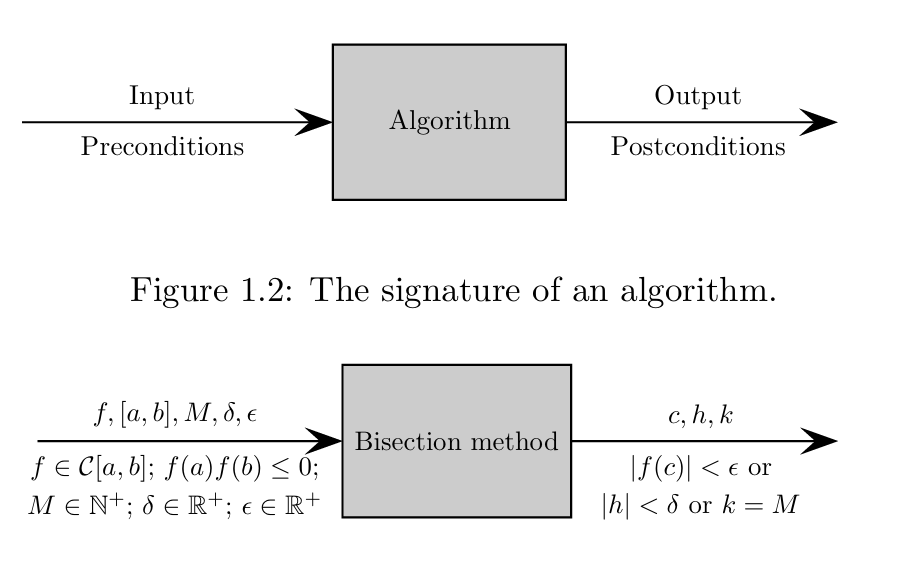
\includegraphics[width=0.75\textwidth]{images/algorithm_sign.png} % Replace with actual diagram if needed
\caption{算法的签名结构图}
\label{fig::signature}
\end{figure}

\begin{remark}
    % remark 1.3
    \label{rem::contract}
一个算法,就像一个定理,可以被看作是一个\textbf{契约(contract)}:它表示“只要你(用户)给予满足前提条件的输入,我(开发者)就会给你满足后置条件的输出。” 
一个算法可以如图~\ref{fig::signature} 所示地形式化表示。例如,二分法如图~\ref{fig::bisection} 所示。

契约,或者说断言。在定理场合,只要前提条件成立,结论就成立;在算法场合,只要输入符合前置条件,算法就会产生符合后置条件的输出。
\end{remark}

\begin{remark}
    % remark 1.4
如果先决条件被违反,算法的行为或输出将是未定义的。为了确保先决条件成立,我们可以在算法内部显式地检查它们(通常用关键字 \textbf{check} 表示),
或者将此责任转交给用户(通常用关键字 \textbf{require} 表示)。

在测试程序时,其本质是:在输入满足先决条件的测试用例后,验证后置条件是否成立。

定理需要被证明,而理论上讲,一个算法作为一个断言,也是可以被证明的,或者,作为在一个有限精度计算机上的程序,可以被测试,甚至被遍历测试。
\end{remark}

\begin{definition}
算法的签名由以下部分组成:输入、输出、前置条件、后置条件,以及对不满足前置条件的输入参数的处理方式。
\end{definition}

\begin{remark}
一个算法的签名从“黑箱”的外部唯一地决定了它的行为。
\end{remark}


\subsection{算法的正确性证明与简化}

\begin{definition}
\textbf{不变量}(invariant)是指在算法执行过程中始终成立的条件。
\end{definition}

\begin{remark}
算法的三个基本构建模块是:顺序执行的简单语句、条件语句,以及循环语句。我们特别关注的是那些在循环过程中保持不变的不变量。
\end{remark}

\begin{definition}
若某个变量在循环体内初始化,则称其为\textbf{临时变量}或\textbf{派生变量};若某个变量在进入循环之前就已初始化,并在不同迭代中保持其值的变化,
则称其为\textbf{持久变量}或\textbf{主变量}。    
\end{definition}

\begin{exercise}
算法 \ref{alg::bisection} 中的不变量有哪些?变量 \(a, b, c, h, u, v, w\) 各自表示什么?哪些是主变量?哪些是临时变量?请画出图示来说明这些变量的生命周期。    
\end{exercise}

\begin{remark}
为了证明一个算法的正确性,我们必须说明:
\begin{itemize}
  \item 算法在有限时间内终止;
  \item 输出满足后置条件。
\end{itemize}

第二点通常通过主变量的不变量,以及派生变量对主变量的依赖关系来证明。
\end{remark}

\begin{remark}
针对备注 \ref{rem::contract} 中的类比,我们关注的是黑箱的外部。事实上,该类比也适用于黑箱的内部,
含义如下:就像我们在证明定理时不需要无关或冗余的参数一样,我们也应尽可能简化算法。
\end{remark}

\begin{algorithm}
    % alg 1.9
    \label{alg::simple_bisection}
简化的二分法算法:

\begin{minipage}{0.45\textwidth}
\textbf{输入:} \\
$f : [a,b] \rightarrow \mathbb{R}$,$a \in \mathbb{R}$,$b \in \mathbb{R}$ \\
$M \in \mathbb{N}$,$\delta \in \mathbb{R}^+$,$\epsilon \in \mathbb{R}^+$ \\
\textbf{前提条件:} \\
$f \in C([a,b])$, $\text{sgn}(f(a)) \neq \text{sgn}(f(b))$ \\
\textbf{输出:} $c, h, k$ \\
\textbf{后置条件:} $|f(c)| < \epsilon$ 或 $|h| < \delta$ 或 $k = M$
\end{minipage}

\begin{enumerate}
\item $h \leftarrow b - a$
\item $u \leftarrow f(a)$
\item \textbf{for} $k = 0$ \textbf{to} $M$
\item \quad $h \leftarrow h / 2$
\item \quad $c \leftarrow a + h$
\item \quad \textbf{if} $|h| < \delta$ 或 $k = M$ \textbf{then break}
\item \quad $w \leftarrow f(c)$
\item \quad \textbf{if} $|w| < \epsilon$ \textbf{then break}
\item \quad \textbf{else if} $\text{sgn}(w) = \text{sgn}(u)$ \textbf{then}
\item \qquad $a \leftarrow c$
\item \textbf{end for}
\end{enumerate}
    
\end{algorithm}

\begin{remark}
如果将第 2 行放置在循环开始之后的位置,将更容易证明算法 \ref{alg::simple_bisection} 的正确性。
在这种情况下,证明可以基于以下两点:
\begin{enumerate}
    \item 观察到只有变量 \(a\) 是主变量,其他变量都是由 \(a\) 推导而来;
    \item 区间长度在每次迭代中都会缩小为原来的一半,这构成了一个不变量。
\end{enumerate}
此外,将第 2 行放在循环外并不会影响算法的正确性,因为在循环中我们只需要用到 \(f(a)\) 的符号。
\end{remark}

\begin{remark}
    % rem 1.10
    \label{rem::reduce_cost}
第 2 行留在循环之外的另一个重要原因是:计算非线性函数 \(f\) 可能代价较高。换句话说,我们应尽量减少在二分法循环中对 \(f\) 的求值。

事实上,只有当算法 \ref{alg::bisection} 和算法 \ref{alg::simple_bisection} 在循环中对 \(f\) 的求值次数相同,
它们在效率上才具有可比性。这也是两个算法中第 6 行的条件语句为何要与第 8 行分开的原因。
\end{remark}

\begin{remark}
算法 \ref{alg::simple_bisection} 相较于算法 \ref{alg::bisection},有哪些方面更加简单?
总的代码行数并不重要,一个更好的衡量方式是主变量的数量:算法 \ref{alg::bisection} 有四个主变量,而算法 \ref{alg::simple_bisection} 只有两个。

此外,算法 \ref{alg::simple_bisection} 中的主变量 \(h\) 是非常可预测的(在每次循环中都除以 $2$),
因此我们实际上只有一个主变量在语法结构和语义上都真正重要。
\end{remark}


\subsection{Q-阶收敛性}
% subsec 1.4
\label{subsec::Q_convergence}

\begin{definition}
    % def 1.10
    \label{def::Q_convergence}
(Q-阶收敛性)一个收敛序列 \(\{x_n\}\) 若满足以下条件,则称其以 Q-阶 \(p\)(其中 \(p \ge 1\))收敛于 \(L\):
\begin{equation}
\lim_{n \to \infty} \frac{|x_{n+1} - L|}{|x_n - L|^p} = c > 0
\end{equation}
其中常数 \(c\) 被称为\textbf{渐近因子(asymptotic factor)}。特别地:
\begin{itemize}
    \item 若 \(p = 1\),称为\textbf{线性收敛};
    \item 若 \(p = 2\),称为\textbf{二次收敛}。
\end{itemize}    
\end{definition}

\begin{remark}
收敛阶衡量的是收敛的速度。然而,只有当一个数列被证明确实收敛时,我们才能称其具有 $Q$ 阶收敛。换句话说,
定义 \ref{def::Q_convergence} 并不保证收敛,它仅仅衡量收敛的速度。

以求解 \( f(x) = \sin(x) = 0 \) 且 \( x \) 接近 $3$ 的情形为例。
如果渐近因子 \( c = 0.1 \), 那么线性收敛方法的每一次迭代将带来一位新的有效数字。如果 \( c = \frac{1}{2} \),
那么线性收敛方法的每次迭代将带来一位新的有效比特。对于二次收敛方法,每次迭代大致会使正确的数字或比特数翻倍。
\end{remark}

\begin{definition}
    % def 1.11
    \label{def::linear_convergence}
序列 \(\{x_n\}\) 若满足:
\begin{equation}
    % eq 1.2
    \label{eq::linear_convergence}
\exists c \in (0, 1), \exists d > 0, \text{使得 } \forall n \in \mathbb{N}, \quad |x_n - L| \le c^n d
\end{equation}
则称其\textbf{线性收敛于} \(L\).

若收敛序列 \(\{x_n\}\) 满足:
\begin{equation}
    % eq 1.3
    \label{eq::Q_convergence}
\exists c > 0, \exists N \in \mathbb{N}, \text{使得 } \forall n > N, \quad |x_{n+1} - L| \le c|x_n - L|^p
\end{equation}
则称其具有 \(p\) 阶收敛。  
\end{definition}

\begin{remark}
定义 \ref{def::linear_convergence} 可由定义 \ref{def::Q_convergence} 推出。(请使用定义 C.3 来证明这一点!)

请注意,(\ref{eq::linear_convergence}) 同时也保证了收敛性,而 (\ref{eq::Q_convergence}) 并不保证。例如,数列 \(\{1, -1, 1, -1, \dots\}\) 
满足 (\ref{eq::Q_convergence}) 中 \(L = 0\)、\(p = 1\)、\(c = 1\) 的条件,但该数列并不收敛。

(\ref{eq::linear_convergence}) 保证收敛性的关键在 于 \(c < 1\),而 (\ref{eq::Q_convergence}) 中的 \(c\) 可以大于 $1$.
\end{remark}

\begin{theorem}
(单调收敛定理)任何有界的单调序列都是收敛的。
\end{theorem}

\begin{theorem}
    % thm 1.13
    \label{thm::bisection}
(二分法的收敛性)设函数 \(f : [a_0, b_0] \to \mathbb{R}\) 连续,且满足 \(\text{sgn}(f(a_0)) \neq \text{sgn}(f(b_0))\),则二分法中迭代序列的误差以因子 \(\frac{1}{2}\) 线性收敛:
\begin{equation}
\lim_{n \to \infty} a_n = \lim_{n \to \infty} b_n = \lim_{n \to \infty} c_n = \alpha
\end{equation}
\begin{equation}
f(\alpha) = 0
\end{equation}
\begin{equation}
|c_n - \alpha| \le 2^{-n+1}(b_0 - a_0)
\end{equation}
其中 \([a_n, b_n]\) 表示第 \(n\) 次迭代的区间,\(c_n = \frac{1}{2}(a_n + b_n)\) 为当前迭代的中点。    
\end{theorem}

\begin{proof}
由算法定义可知:
\[
a_0 \le a_1 \le a_2 \le \cdots \le \alpha,\quad
b_0 \ge b_1 \ge b_2 \ge \cdots \ge \alpha
\]
\[
b_{n+1} - a_{n+1} = \frac{1}{2}(b_n - a_n)
\]
由单调收敛定理,\(\{a_n\}, \{b_n\}\) 均收敛,且区间长度趋于 $0$,因此中点也收敛于某个 \(\alpha\)。
由算法和初始条件可知,每次迭代区间内 \(f(a_n)f(b_n) \le 0\) 成立,故 \(f(\alpha) = 0\).
\end{proof}

\begin{remark}
请注意算法 \ref{alg::bisection} 的表示方式和循环\textit{不变量}是如何在定理 \ref{thm::bisection} 的证明中被利用的。
\end{remark}

\begin{remark}
二分法的优点包括:保证收敛、最终误差明确,并且易于并行计算。其缺点是收敛速度较慢,且在寻找满足 \( f(a)f(b) < 0 \) 的两个点 \(a, b\) 时可能存在困难。
这些观察基于一个事实:在许多实际情形中,我们可能并不知道函数 \(f(x)\) 的精确形式。
\end{remark}

\subsection{牛顿法}
\begin{remark}
    我们已经有二分法了,为何需要更多的方法?
\end{remark}

来看一个本质上快于二分法的求根算法, 因为它是 $Q$-二阶的, 而二分法是
$Q$-线性的. 它的来源是对 $f$ 在真解 $x^*$ 处做关于初值 $x_0$ 的 Taylor
展开, 并截断到第二项:
\begin{eqnarray*}
  &&0 = f(x^*)=f(x_0)+(x^* - x_0)f'(x_0) + o((x^* - x_0)^2) \\
  &\Rightarrow&f(x_0) + x^*f'(x_0) - x_0f'(x_0) \approx 0 \\
  &\Rightarrow&x^* \approx x_0 - \frac{f(x_0)}{f'(x_0)}.
\end{eqnarray*}
由此得到迭代公式.

\begin{figure}
\centering
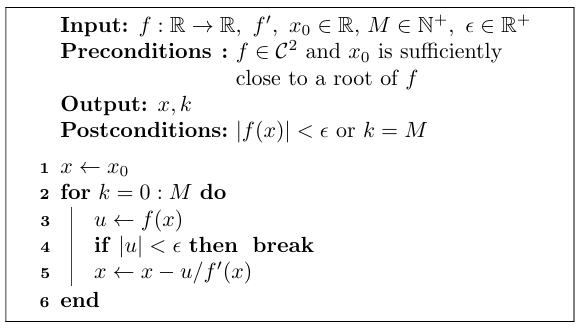
\includegraphics[width=0.75\textwidth]{images/newton_method.png}
\caption{牛顿法的步骤}    
\label{fig::newton}
\end{figure}

\begin{algorithm}
    % alg 1.14
    \label{alg::newton}
如图 \ref{fig::newton} 和 \ref{fig::geo_newton} 所示,牛顿法用于求解函数 \(f : \mathbb{R} \rightarrow \mathbb{R}\) 的根,从初始值 \(x_0\) 开始,使用迭代公式:
\begin{equation}
    % 
    \label{eq::newton}
x_{n+1} = x_n - \frac{f(x_n)}{f'(x_n)}, \quad n \in \mathbb{N}
\end{equation}
\end{algorithm}

\begin{remark}
一个函数的自变量可以包含另一个函数。这种特殊类型的函数被称为 \textit{泛函}(functional)或 \textit{函数子}(functor). 
在 \textbf{matlab} 中,函数子通过函数指针 \texttt{@} 实现;在 \textbf{C++} 中,函数子是具有 \texttt{operator()} 的类。
\end{remark}

\begin{remark}
牛顿法收敛得非常快,以至于在二分法中所需的停止准则 \(\delta\) 并不是必须的。
\end{remark}

\begin{figure}
\centering
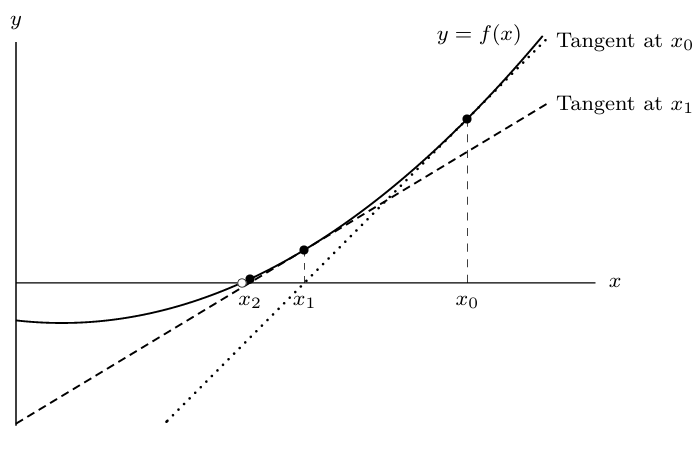
\includegraphics[width=0.75\textwidth]{images/geo_newton.png}
\caption{牛顿法的几何解释}
\label{fig::geo_newton}
\end{figure}

\begin{theorem}
    % 1.15
    \label{thm::newton}
(牛顿法的收敛性)  
设 \( f : \mathcal{B} \to \mathbb{R} \) 是定义在区间 \( \mathcal{B} = [\alpha - \delta, \alpha + \delta] \) 上的 \( C^2 \) 函数,
满足 \( f(\alpha) = 0 \) 且 \( f'(\alpha) \ne 0 \). 
若初始点 \( x_0 \) 足够接近根 \(\alpha\),则牛顿法生成的迭代序列 \(\{x_n\}\) 至少以\textbf{二次速度}收敛于 \(\alpha\),即:
\begin{equation}
\lim_{n \to \infty} \frac{\alpha - x_{n+1}}{(\alpha - x_n)^2} = \frac{f''(\alpha)}{2f'(\alpha)}.     
\end{equation}    
\end{theorem}

\begin{proof}
由泰勒公式(定理 C.99)和 \(f \in C^2\) 得:
\[
f(\alpha) = f(x_n) + (\alpha - x_n) f'(x_n) + \frac{(\alpha - x_n)^2}{2} f''(\xi)
\]
其中 \(\xi\) 在 \(x_n\) 与 \(\alpha\) 之间。因为 \(f(\alpha) = 0\),代入得:
\[
- \alpha = - x_n - \frac{f(x_n)}{f'(x_n)} + \frac{(\alpha - x_n)^2}{2} \frac{f''(\xi)}{f'(x_n)}
\]
即:
\[
x_{n+1} - \alpha = (x_n - \alpha)^2 \cdot \frac{f''(\xi)}{2f'(x_n)} \tag{*}
\]
由 \(f'(\alpha) \ne 0\) 的连续性可知,存在 \(\delta \in (0, \delta)\),使得在集合 
\(\mathcal{B}_1 = [\alpha - \delta_1, \alpha + \delta_1]\) 中,\(f'(x)\) 有界且不为零。
设:
\[
M := \frac{\max_{x \in \mathcal{B}_1} |f''(x)|}{2 \min_{x \in \mathcal{B}_1} |f'(x)|}
\]
若初始点 \(x_0\) 满足:
\begin{itemize}
    \item[(i)] \(|x_0 - \alpha| = \delta_0 < \delta_1\);
    \item[(ii)] \(M \delta_0 < 1\).
\end{itemize}
则根据 (*) 式可得:
\[
|x_{n+1} - \alpha| \le M |x_n - \alpha|^2
\]
所以收敛阶为 $2$. 并且由归纳法可得:
\[
|x_n - \alpha| \le \frac{1}{M} (M |x_0 - \alpha|)^{2^n}
\]
即 $x_n$ 收敛至 $\alpha$. 这证明了二次收敛性。若 \(f''(\alpha) = 0\),收敛速率可能高于二次。 
\end{proof}

\begin{remark}
短语 “至少”(at least)指的是超收敛情形,即 \( f''(\alpha) = 0 \). 
定理 \ref{thm::newton} 中模糊的表达 “足够接近”(sufficiently close)指的是其证明中条件 (i)、(ii),这两个条件必须同时满足。

换句话说,我们并没有一个逐步构造 \( x_0 \) 来满足这些条件的方法;我们甚至不会去尝试。
为什么?因为我们对函数 \( f \) 的信息不足。我们所能做的最好的事情,就是要求条件 (i)、(ii) 同时成立。
\end{remark}

\begin{remark}
牛顿法的主要优点是其收敛速度非常快。其缺点之一是需要我们知道导数 \( f'(x) \), 
而这可能难以获得,或者计算起来耗时较长。牛顿法的另一个主要缺点是我们无法判断初始点 \( x_0 \) 是否足够接近真实根。因此,收敛性无法得到保证。

例如,如果在定理 \ref{thm::newton} 的证明中条件 (i) 被违反,那么下一次迭代可能会远离根 \(\alpha\). 图 \ref{fig::newton_cond} 展示了条件 (ii) 的必要性。
\end{remark}

\begin{figure}
    % fig 1.6
    \label{fig::newton_cond}
\centering
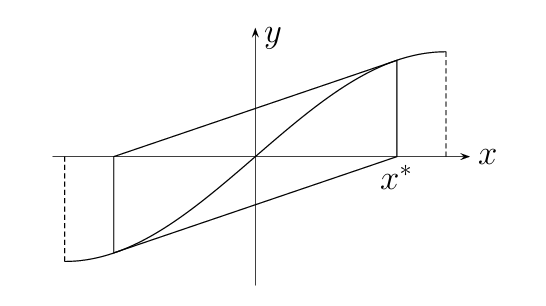
\includegraphics[width=0.5\textwidth]{images/newton_cond.png} % Replace with actual image
\caption{展示定理 \ref{thm::newton} 中条件必要性的特殊例子}
\end{figure}

\begin{theorem}
    % 1.16
    \label{thm::monotone}
若连续函数 \(f: [a,b] \to [c,d]\) 是双射,当且仅当 \(f\) 是严格单调的。
\end{theorem}

\begin{remark}
定理 \ref{thm::monotone} 的充分性部分可以重述为:“如果函数 \( f : [a, b] \to [c, d] \) 是连续且严格单调的,那么它是双射(bijective)。”\\
但其逆命题并不成立。你能给出一个反例吗?
\end{remark}

\begin{remark}
我们注意到,由于缺乏对函数 \( f \) 的信息,牛顿法的收敛性无法得到保证。解决该问题的一种方法是对 \( f \) 施加更多条件;定理 \ref{thm::newton_monotone} 就是一个例子。
\end{remark}

\begin{theorem}
    % thm 1.17
    \label{thm::newton_monotone}    
若 \(f : \mathbb{R} \to \mathbb{R}\) 为 \(C^2\) 函数,满足:
\begin{itemize}
    \item \(f(\alpha) = 0\)
    \item \(f' > 0\), \(f'' > 0\)
    \item \(\alpha\) 是 \(f\) 的唯一根
\end{itemize}
则对于任意 \(x_0 > \alpha\), 牛顿法迭代序列 \(\{x_n\}\) 二次收敛于 \(\alpha\).    
\end{theorem}

\begin{proof}
由定理 \ref{thm::monotone} 可知,函数 \( f \) 是双射,因为 \( f \) 是连续且严格单调的。
由于 \( 0 \) 在其值域中,\( f \) 必有唯一根。在证明定理 \ref{thm::newton} 时,我们有:

\begin{equation}
    % eq 1.9
    \label{eq::newton_residual}
x_{n+1} - \alpha = (x_n - \alpha)^2 \cdot \frac{f''(\xi)}{2 f'(x_n)}. 
\end{equation}

进一步地,\( f' > 0 \) 且 \( f'' > 0 \) 意味着对所有 \( n > 0 \), 
都有 \( x_n > \alpha \). 由于 \( f \) 是严格递增的,意味着 \( f(x_n) > f(\alpha) = 0 \), 
对所有 \( n > 0 \) 成立。根据牛顿法的定义,

\[
x_{n+1} - \alpha = x_n - \alpha - \frac{f(x_n)}{f'(x_n)},
\]

因此序列 \( \{x_n - \alpha : n > 0\} \) 是严格单调递减的,且以 $0$ 为下界。
由定理 \ref{eq::secant} 可知,该序列收敛。

设 \( \lim_{n \to \infty} x_n = a \),两边对等式 (\ref{eq::newton}) 取极限得:

\[
a = a - \frac{f(a)}{f'(a)},
\]

由此可得 \( f(a) = 0 \). 由于 \( f \) 的根是唯一的,因此 \( a = \alpha \)。

二次收敛速率可使用等式 (\ref{eq::newton_residual}) 进行归纳证明,如同在定理 \ref{thm::newton} 中所做的那样。
\end{proof}

\begin{remark}
对牛顿迭代 \( (x_n)_{n \in \mathbb{N}} \) 唯一收敛于 \(\alpha\) 的证明如下。

假设数列 \(\{x_n\}\) 收敛于 \(\alpha + c\),其中 \(c > 0\) 为某个固定常数。定义:
\[
\delta = \frac{f(\alpha + c)}{f'(\alpha + c)}.
\]
将 \(f(\alpha + c)\) 在 \(\alpha\) 处展开为泰勒级数,结合 \(f'(\alpha + c) > 0\) 可知 \(\delta > 0\)。因为牛顿迭代 \(\{x_n\}\) 收敛,所以有:
\[
\forall \epsilon > 0,\ \exists N \in \mathbb{N},\ \text{使得} \ \forall n > N,\ |x_n - x_{n+1}| = \left| \frac{f(x_n)}{f'(x_n)} \right| < \epsilon,
\]
尤其当 \(\epsilon = \frac{1}{2} \delta\) 时成立。

另一方面,
\[
\left| x_n - x_{n+1} - \frac{f(\alpha + c)}{f'(\alpha + c)} \right|
\geq \left| x_n - x_{n+1} \right| - \left| \frac{f(\alpha + c)}{f'(\alpha + c)} \right|
> \delta - \frac{1}{2} \delta = \frac{1}{2} \delta = \epsilon.
\]

这与牛顿迭代 \(\{x_n\}\) 收敛于 \(\alpha + c\) 的假设矛盾。因此结合前面的推理,说明牛顿迭代 \(\{x_n\}\) 实际上收敛于 \(\alpha\),即 \(f\) 的唯一根。
\end{remark}

\begin{definition}
向量空间 \(V\) 的子集 \(\mathcal{U}\) 是凸集当且仅当:
\begin{equation}
\forall x, y \in \mathcal{U}, \forall t \in (0,1), \quad tx + (1 - t)y \in \mathcal{U} 
\end{equation}
即线段上的所有点都在集合中。    
\end{definition}

\begin{definition}
函数 \(f : \mathcal{U} \to \mathbb{R}\) 是凸函数当且仅当:

\begin{equation}
    % eq 1.11
    \label{eq::convex_function}
\forall x, y \in \mathcal{U}, \forall t \in (0,1), \quad f(tx + (1 - t)y) \le t f(x) + (1 - t) f(y) 
\end{equation}    
\end{definition}

若将 \ref{eq::convex_function} 中“\(\le\)”换为“\(<\)”,则称 \(f\) 为严格凸函数。


\begin{remark}
一个 \( C^2 \) 函数 \( f : I \to \mathbb{R} \) 是凸的,当且仅当 \( f'' \geq 0 \) 在区间 \( I \) 上成立。
我们现在可以看到,定理 \ref{thm::newton_monotone} 中对函数 \( f \) 的要求是严格单调性和严格凸性。
\end{remark}

\begin{remark}
牛顿法可以通过反函数定理 D.120 直接推广到非线性方程组的情形;参见备注 D.53。
\end{remark}

\subsection{割线法}

\begin{remark}
如前所述,计算导数 \( f'(x) \) 可能代价非常高。为了降低计算成本,我们可以重复利用 \( x_n \) 和 \( x_{n-1} \) 处的函数值来近似导数。
这正是弦截法(secant method)的核心思想,它通常具有较高的性价比。
\end{remark}

\begin{algorithm}
如图~\ref{fig::secant-alg} 所示,割线法用于在初始猜测 \( x_0, x_1 \) 附近求解函数 \( f : \mathbb{R} \to \mathbb{R} \) 的根,其迭代公式为:
\begin{equation}
    % eq 1.12
    \label{eq::secant}
x_{n+1} = x_n - f(x_n) \frac{x_n - x_{n-1}}{f(x_n) - f(x_{n-1})}, \quad n \in \mathbb{N}^+.
\end{equation}
    
\end{algorithm}

\begin{figure}
\centering
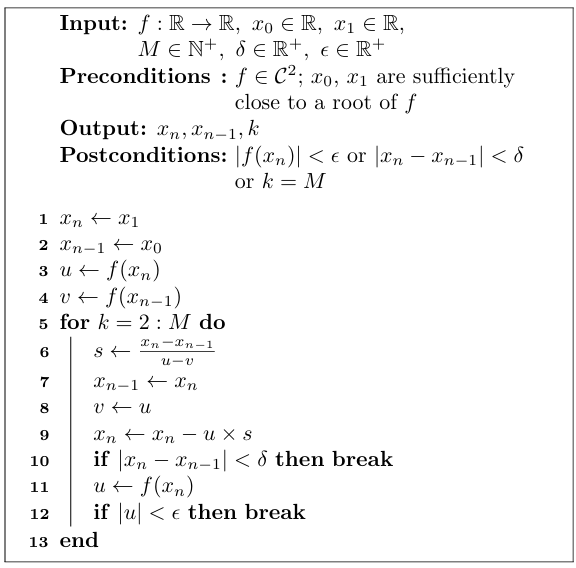
\includegraphics[width=0.75\textwidth]{images/secant_method.png} % 替换为实际图像
\caption{割线法算法}
\label{fig::secant-alg}
\end{figure}

\begin{remark}
我们将第 10 行的条件判断与第 12 行的分开,以减少对非线性函数的求值次数;参见备注 \ref{rem::reduce_cost}。
\end{remark}

\begin{definition}
    % 1.21
    \label{def::fibonacci}
斐波那契数列 \( \{F_n\} \) 定义为:
\begin{equation}
    % eq 1.13
    \label{eq::fibonacci}
F_0 = 0, \quad F_1 = 1, \quad F_{n+1} = F_n + F_{n-1}.
\end{equation}
\end{definition}

\begin{theorem}[Binet 公式]
    % 1.22
    \label{thm::binet}
设黄金比例为 \( r_0 = \frac{1+\sqrt{5}}{2} \),其共轭根为 \( r_1 = 1 - r_0 = \frac{1 - \sqrt{5}}{2} \),则斐波那契数列可表示为:
\begin{equation}
    % eq 1.14
F_n = \frac{r_0^n - r_1^n}{\sqrt{5}}.
\end{equation}
\end{theorem}

\begin{proof}
由定义 \ref{def::fibonacci} 可得:

令
\[
\mathbf{u}_k := 
\begin{bmatrix}
F_{k+1} \\
F_k
\end{bmatrix},
\quad
A := 
\begin{bmatrix}
1 & 1 \\
1 & 0
\end{bmatrix},
\]
则有 \( \mathbf{u}_k = A^k \mathbf{u}_0 \)。因此特征方程为:
\[
\det(A - \lambda I) = \lambda^2 - \lambda - 1 = 0
\]
其根为 \( r_0, r_1 \)。设对应特征向量为 \( \mathbf{x}_0, \mathbf{x}_1 \),则
\[
\mathbf{u}_0 = \frac{1}{r_0 - r_1} (r_0 \mathbf{x}_0 - r_1 \mathbf{x}_1)
\]
代入得结果。
\end{proof}

\begin{remark}
由于 \( r_0 \approx 1.618 \), \( r_1 \approx -0.618 \), 我们有
\[
\lim_{n \to +\infty} \left(F_n - \frac{r_0^n}{\sqrt{5}}\right) = 0.
\]
为了用浮点数计算 \( F_n \), 可以先计算 \( r_0^n / \sqrt{5} \), 再将结果四舍五入为最接近的整数以得到 \( F_n \). 
然而,这种方法可能比直接使用公式 (\ref{eq::fibonacci}) 计算慢得多。为什么?
\end{remark}

\begin{corollary}
    % 1.23
    \label{cor::fib_recurrence}
定理 \ref{thm::binet} 中的 \( r_0, r_1 \) 满足:
\begin{equation}
    % eq 1.15
F_{n+1} = r_0 F_n + r_1^n.
\end{equation}
\end{corollary}

\begin{lemma}[割线法误差表达式]
    % 1.24
    \label{lem::secant_error}
对于割线法(\ref{eq::secant}),存在 \( \xi_n \in (x_{n-1}, x_n) \), 
\( \zeta_n \in \big( \min(x_{n-1}, x_n, \alpha), \max(x_{n-1}, x_n, \alpha) \big) \), 使得:
\begin{equation}
    % eq 1.16
x_{n+1} - \alpha = (x_n - \alpha)(x_{n-1} - \alpha) \cdot \frac{f''(\zeta_n)}{2 f'(\xi_n)}.
\end{equation}
\end{lemma}

\begin{proof}
定义差商为:
\begin{equation}
    % eq 1.17
f[a,b] = \frac{f(a) - f(b)}{a - b}.
\end{equation}

代数变换可得公式等价为:
\begin{equation}
    % eq 1.18
x_{n+1} - \alpha = (x_n - \alpha)(x_{n-1} - \alpha) \cdot \frac{f[x_n, x_{n-1}] - f[x_n, \alpha]}{f[x_{n-1}, x_n]}.
\end{equation}

由平均值定理存在 \( \xi_n \in (x_{n-1}, x_n) \) 使得:
\begin{equation}
    % eq 1.19
f[x_{n-1}, x_n] = f'(\xi_n)
\end{equation}

定义 \( g(x) := f[x, x_n] \),再应用平均值定理,有:
\begin{equation}
    % eq 1.20
\frac{f[x_n, x_{n-1}] - f[x_n, \alpha]}{x_{n-1} - \alpha} = g'(\beta)
\end{equation}

对 \( g'(x) \) 求导并使用拉格朗日余项公式,有:
\begin{equation}
    % eq 1.21
\frac{f[x_n, x_{n-1}] - f[x_n, \alpha]}{x_{n-1} - \alpha} = \frac{f''(\zeta_n)}{2}
\end{equation}
代入即得结论。
\end{proof}

\begin{theorem}[割线法收敛性]
    % 1.25
    \label{thm::secant}
设函数 \( f : \mathcal{B} \to \mathbb{R} \) 为 \( C^2 \) 函数,
定义在区间 \( \mathcal{B} = [\alpha - \delta, \alpha + \delta] \) 上,
满足 \( f(\alpha) = 0 \)、\( f'(\alpha) \ne 0 \)、\( f''(\alpha) \ne 0 \),
若初始点 \( x_0, x_1 \) 足够接近 \(\alpha\),则割线法迭代序列 \( \{x_n\} \) 收敛于 \(\alpha\),其收敛阶为:
\begin{equation*}
    \label{eq::golden_ratio}
p = \frac{1 + \sqrt{5}}{2} \approx 1.618.
\end{equation*}
\end{theorem}

\begin{proof}
由于 \( f' \) 连续,且 \( f'(\alpha) \ne 0 \),可得存在 \( \delta_1 \in (0, \delta) \),
使得对所有 \( x \in \mathcal{B}_1 \subseteq \mathcal{B} \),有 \( f'(x) \ne 0 \).
其中 \( \mathcal{B}_1 = [\alpha - \delta_1, \alpha + \delta_1] \). 
定义 \( E_i = |x_i - \alpha| \),
\[
M = \frac{\displaystyle \max_{x \in B_1} |f''(x)|}{\displaystyle 2 \min_{x \in B_1} |f'(x)|}
\]
由引理 \ref{lem::secant_error} 可得:
\begin{equation*}
ME_{n+1} \leq ME_n ME_{n-1}.
\end{equation*}

选择初始点 \(x_0, x_1\) 满足:

\begin{enumerate}
    \item \( E_0 < \delta, \quad E_1 < \delta \);
    \item \( \max(ME_1, ME_0) = \eta < 1 \).
\end{enumerate}

则根据上述递推关系,可由归纳法证明:存在 \(\eta\) 使得所有 \( ME_n < \eta \). 记 \( ME_0 \leq \eta \),
 \( ME_1 \leq \eta \), 
 \( ME_2 \leq ME_1 ME_0 \leq \eta^2 \), 
 \( ME_3 \leq ME_2 ME_1 \leq \eta^3 \), $\cdots$, 
 \( ME_{n + 1} \leq ME_n ME_{n - 1} \leq \eta^{F_n + F_{n - 1}} = \eta^{F_n} \), 
 以此类推,得:
\[
E_n \leq B_n := \frac{1}{M} \eta^n.
\]
由定理 \ref{thm::binet} 可得:
\[
q_n \to \frac{1.618^{n+1}}{\sqrt{5}},
\]
从而 \( \lim_{n \to \infty} E_n = 0 \).

为了估计收敛速率,首先研究上界 \( \{B_n\} \) 的下降速度:

\begin{equation*}
\frac{B_{n+1}}{B^{r_0}_n} = \frac{\left(\frac{1}{M}\right)\eta^{F_{n+1}}}{\left(\frac{1}{M}\right)^{r_0}\eta^{r_0F_{n}}} 
= M^{r_0 - 1} \eta^{F_{n + 1} - r_0 F_n} \leq M^{r_0 - 1} \eta^{-1},
\end{equation*}
注意由推论 \ref{cor::fib_recurrence}  \( F_{n+1} - r_0 F_n = r_1^{n} \to -1 \). 

为证明收敛速率,我们定义:
\begin{equation}
    % eq 1.22
m_n := \frac{f''(\zeta_n)}{2f'(\xi_n)}, \quad m_\alpha := \left| \frac{f''(\alpha)}{2f'(\alpha)} \right|,
\end{equation}

其中 \( \zeta_n, \xi_n \) 与引理 \ref{lem::secant_error} 中相同。

通过归纳法,我们有:
\begin{align*}
E_n &= E_1^{{F_n}} E_0^{{F_{n-1}}} m_1^{F_{n-1}} \cdots m_{n-1}^{F_1}, \\
E_{n+1} &= E_1^{F_{n+1}} E_0^{F_n} m_1^{F_n} \cdots m_n^{F_1},
\end{align*}

其中 \( F_n \) 是定义 \ref{def::fibonacci} 中的斐波那契数列。于是,

\begin{equation}
    % eq 1.23
    \begin{array}{rcl}
\frac{E_{n+1}}{E_0^{F_n}} &=& E_1^{F_{n+1} - r_0 F_n} E_0^{F_n - r_0 F_{n-1}} m_1^{F_n - r_0 F_{n-1}} \cdots m_n^{F_1 - r_0 F_0}, \\
&=& E_1^{F_{n+1} - r_0 F_n} E_0^{F_n - r_0 F_{n-1}} \prod_{j=1}^n m_j^{F_{n+1-j} - r_0 F_{n-j}}, \\
&=& E_1^{r_1^{n-1}} E_0^{r_1^{n-2}} \cdots m_1^{r_1^1} m_n^{r_1^n}.
    \end{array}
\end{equation}

由推论 \ref{cor::fib_recurrence} 可得:

% \begin{equation}
%     % eq 1.24
% \lim_{n \to \infty} \frac{E_{n+1}}{E_0^{F_n}} = \lim_{n \to \infty} A \cdot \lim_{n \to \infty} B 
% = \lim_{n \to \infty} B \leq 2^{r_1 + r_1^2 + \cdots} \cdot \frac{1}{m_\alpha^0}.
% \end{equation}

\begin{equation}
    % eq 1.24
\lim_{n \to \infty} m_n = m_\alpha,
\end{equation}

于是存在常数 \( N \in \mathbb{N} \),使得对所有 \( n > N \),有:
\begin{equation}
    % eq 1.25
m_n \in \left( \frac{1}{2} m_\alpha, 2m_\alpha \right)
\end{equation}

定义:
\begin{equation*}
A := E_1^{r_1^{n-1}} E_0^{r_1^{n-2}} \cdots m_1^{r_1^1} m_2^{r_1^2} \cdots m_{N}^{r_1^N}
\end{equation*}

\begin{equation*}
B := m_{N+1}^{r_1^{N+1}} \cdots m_n^{r_1^n}
\end{equation*}

因此:
\begin{equation*}
\lim_{n \to \infty} B \leq 2^{\sum_{i=N+1}^{\infty} r_1^i} \cdot \frac{1}{m_\alpha^0}
\end{equation*}
\end{proof}

\begin{remark}
尽管牛顿法具有更高的收敛速度,弦截法可能计算代价更低。因此,对于一个给定的问题,我们应如何在牛顿法和弦截法之间做出选择?
如果我们 \textit{事先} 知道所需解的精度,那就选择 \textbf{CPU 时间更少} 的方法。
\end{remark}

\begin{corollary}
    % 1.26
    \label{cor::newton_secant_time}
若考虑 \( f(x) = 0 \) 在 \( x = \alpha \) 处的根,记 \( m \) 和 \( sm \) 分别为评估 \( f(x) \) 与 \( f'(x) \) 所需的时间,则达到所需精度所需的最短迭代次数分别为:

\begin{equation}
    % eq 1.26
    \label{eq::newton_secant_time}
T_N = (1 + s)m \lceil \log_2 K \rceil,
\end{equation}

\begin{equation}
    % eq 1.27
T_S = m \lceil \log_{r_0} K \rceil + m,
\end{equation}

其中:
\begin{equation*}
r_0 = \frac{1 + \sqrt{5}}{2}, \quad c = \left| \frac{f''(\alpha)}{2f'(\alpha)} \right|,
\end{equation*}

\begin{equation}
    % eq 1.28
K = \frac{\log c}{\log |x_0 - \alpha|},
\end{equation}

符号 \( \lceil \cdot \rceil \) 表示向上取整。
\end{corollary}

\begin{proof}
在定理 \ref{thm::newton} 中我们已证明 \( |x_n - \alpha| \leq \frac{1}{M} (ME_0)^{2^n} \), 令 \( E_n = |x_n - \alpha| \), 则有:
\[
ME_n \leq (ME_0)^{2^n}
\]

设 \( i \in \mathbb{N} \) 为最小次数使得误差满足 \( (ME_0)^{2^i} \leq M\epsilon \). 当 \( \epsilon \) 足够小时,\( M \to c \), 因此:

\[
i = \lceil \log_2 K \rceil
\]

对于牛顿法,每轮迭代需要一次函数和导函数评估,总耗时 \( (1 + s)m \). 因此有公式 (\ref{eq::newton_secant_time})。

对于割线法,假设 \( ME_0 \geq ME_1 \)。由定理 \ref{thm::secant} 可得:

\[
ME_n \approx (ME_0)^{\frac{\sqrt{5}}{2} r_0^{n+1}}
\]

忽略指数中的 \( -\frac{\sqrt{5}}{2} r_1^{n+1} \) 项。设 \( j \in \mathbb{N} \) 为最小迭代次数使得误差满足 \( r_0^{\sqrt{5} j} \leq K \), 因此:

\[
j = \left\lceil \frac{\log_{r_0} K + \log_{r_0} \sqrt{5}}{\sqrt{5}} \right\rceil = \lceil \log_{r_0} K \rceil + 1.
\]

由于割线法中初始值 \(x_0\) 和 \(x_1\) 已给出,因此最少迭代次数为 \(\lceil \log_{r_0} K \rceil\)(可与牛顿法比较!)。
此外,由于前一次迭代中已计算 \(f(x_{n-1})\),因此每次迭代仅需计算函数值 \(f(x_n)\)。最后,额外的项 \(m\) 是因为在第一次迭代中还需要计算 \(f(x_0)\).
\end{proof}

\begin{remark}
根据推论 \ref{cor::newton_secant_time},当比值 \( T_S / T_N < 1 \) 时,弦截法比牛顿法更快。这意味着
\[
s > \frac{\log 2}{\log r_0} - 1 \approx 0.44.
\]
\end{remark}

\subsection{不动点迭代}
% subsec 1.7

\begin{definition}
    % 1.27
一个函数 \( g \) 的\textbf{不动点} 是满足 \( g(\alpha) = \alpha \) 的自变量 \(\alpha\).
\end{definition}

\begin{example}
    % 1.28
函数 \( f(x) = x^2 - 3x + 4 \) 的不动点是 \( x = 2 \).
\end{example}

\begin{remark}
对于函数 \( f \) 的一个不动点,我们有
\[
f^n(x) := f(f(\cdots f(x))) = x,
\]
对任意 \( n \in \mathbb{N}^+ \) 成立。因此,这个名称由此而来。
\end{remark}

\begin{lemma}
    % 1.29
    \label{lem::fixed_point}
若 \( g : [a, b] \to [a, b] \) 连续,则 \( g \) 至少在区间 \([a, b]\) 上有一个不动点。
\end{lemma}

\begin{proof}
函数 \( f(x) = g(x) - x \) 满足 \( f(a) \geq 0 \)、\( f(b) \leq 0 \),由介值定理得证。
\end{proof}

\begin{exercise}
    % 1.30
    \label{exe::no_fixed_point}
设 \( A = [-1, 0) \cup (0, 1] \). 给出一个连续函数 \( g : A \to A \), 使其没有不动点。
再给出一个从 \( \mathbb{R} \to \mathbb{R} \) 的连续函数,其同样没有不动点。
\end{exercise}

\begin{remark}
引理 \ref{lem::fixed_point} 和习题 \ref{exe::no_fixed_point} 表明:若一个连续函数的定义域和值域是相同的集合 \( A \), 
在 \( A \) 满足某些条件时,该函数就会有不动点。那么,这些条件是什么呢?布劳威尔不动点定理为我们提供了一些线索。
\end{remark}

\begin{theorem}[Brouwer 不动点定理]
    % 1.31
    \label{thm::brouwer}
设 \( \mathbb{D}^n := \{ x \in \mathbb{R}^n : \|x\| \leq 1 \} \), 则任意连续函数 \( f : \mathbb{D}^n \to \mathbb{D}^n \) 至少有一个不动点。
\end{theorem}

\begin{proof}
见 Milnor [1978]。
\end{proof}

\begin{example}
    % 1.32
将一张地图放在地板上,设函数将地图上的每个点映射到其在地图上的对应位置。若地图是 \( \mathbb{D}^2 \) 的同胚映射,则存在某个点刚好映射到其在地面上的位置。
\end{example}

\begin{exercise}
    % 1.33
将两张相同大小的纸重叠放置,然后揉皱上面的一张纸并压在下面的一张上,证明至少存在一个点在揉皱后仍位于原处。
\end{exercise}

\begin{definition}
    % 1.34
\textbf{不动点迭代} 是通过如下形式迭代寻找不动点的方法:
\begin{equation}
    % eq 1.29
    \label{eq::fixed_point_iteration}
x_{n+1} = g(x_n), \quad n \in \mathbb{N}.
\end{equation}
\end{definition}

\begin{example}
    % 1.35
牛顿法就是一种不动点迭代。
\end{example}

$$
x_{n + 1} = x_n - \frac{f(x_n)}{f'(x_n)},
$$
所以牛顿法的迭代函数为
$$
g(x) = x - \frac{f(x)}{f'(x)}.
$$
它的不动点就是原方程 \( f(x) = 0 \) 的根。



\begin{exercise}
    % 1.36
    \label{exe::fixed_point_behavior}

为计算某个正实数 \( a \) 的平方根,我们可以将问题表述为求函数  
\[f(x) = x^2 - a\]  
的根。  
当 \( a = 1 \), 初始猜测值 \( x_0 = 2 \), 且有以下三种选择:  
\[g_1(x) := x^2 + x - a,\]  
\[g_2(x) := \frac{a}{x},\]  
以及  
\[g_3(x) := \frac{1}{2}\left(x + \frac{a}{x}\right),\]  

这三种形式都是和 $f(x) = 0$ 等价的形式,但可以验证 \( g_1 \) 发散,\( g_2 \) 振荡,\( g_3 \) 收敛。
本节中的定理将解释其原因。
\end{exercise}

\begin{definition}
    % 1.37
    \label{def::contraction}
若函数 \( f : [a, b] \to [a, b] \) 存在 \( \lambda \in [0, 1) \) 使得对任意 \( x, y \in [a, b] \) 有:
\begin{equation}
|f(x) - f(y)| \leq \lambda |x - y|,
\end{equation}
则称 \( f \) 为\textbf{压缩映射(contraction mapping)}。
\end{definition}

\begin{example}
    % 1.38
任意线性函数 \( f(x) = \lambda x + c \),其中 \( 0 \leq \lambda < 1 \),是压缩映射。
\end{example}

\begin{theorem}[压缩映射收敛定理]
    % 1.39
    \label{thm::contraction}
若 \( g(x) \) 是区间 \([a, b]\) 上的压缩映射,则它在 \([a, b]\) 内有唯一的不动点 \( \alpha \). 并且,迭代公式
\[
x_{n+1} = g(x_n)
\]
对于任意初始值 \( x_0 \in [a, b] \) 都收敛于 \( \alpha \),且有误差估计:
\begin{equation}
    % eq 1.31
    \label{eq::contraction_error}
|x_n - \alpha| \leq \frac{\lambda^n}{1 - \lambda} |x_1 - x_0|.
\end{equation}
\end{theorem}

\begin{proof}
由引理 \ref{lem::fixed_point} 知,$g$ 在区间 $[a,b]$ 上至少有一个不动点。设存在两个不同的不动点 $\alpha$ 与 $\beta$, 则
\[
|\alpha-\beta|=|g(\alpha)-g(\beta)|\le \lambda |\alpha-\beta|,
\]
这推出 $|\alpha-\beta|\le 0$, 亦即这两个不动点必相同。

由定义 \ref{def::contraction},$x_{n+1}=g(x_n)$, 从而所有 $x_n$ 都落在 $[a,b]$ 中。
为证明收敛性,注意到
\[
|x_{n+1}-\alpha| = |g(x_n)-g(\alpha)| \le \lambda |x_n-\alpha|.
\]
由归纳法并结合三角不等式,得到
\[
\begin{aligned}
|x_n-\alpha|
&\le \lambda^n |x_0-\alpha| \\
&\le \lambda^n\bigl(|x_1-x_0|+|x_1-\alpha|\bigr) \\
&\le \lambda^n\bigl(|x_1-x_0|+\lambda |x_0-\alpha|\bigr),
\end{aligned}
\]
从而推出
\[
|x_0-\alpha| \le \frac{1}{1-\lambda}\,|x_1-x_0|,
\]
并与式 (\ref{eq::contraction_error}) 一致。
\end{proof}

\begin{remark}
定理 \ref{thm::contraction} 不应与定理 \ref{thm::brouwer} 混淆。关于定理 \ref{thm::contraction} 的一个部分推广,可参见定理 D.118。
\end{remark}

\begin{remark}
有时判断一个函数是否为压缩映射是困难的。另一种方法是检查该函数的导数的绝对值是否 \textbf{处处小于 $1$}.
\end{remark}


\begin{theorem}
    % 1.40
    \label{thm::fixed_point_convergence}
设 $g:[a,b]\to [a,b]$。若 $g\in C^{1}[a,b]$ 且
\[
\lambda=\max_{x\in [a,b]}|g'(x)|<1,
\]
则 $g$ 在区间 $[a,b]$ 内有唯一的不动点 $\alpha$。此外,对任意初值 $x_0\in [a,b]$,不动点迭代式 (\ref{eq::fixed_point_iteration}) 都收敛到 $\alpha$, 
误差估计 (\ref{eq::contraction_error}) 成立,并且
\begin{equation}
    % eq 1.32
    \label{eq::fixed_point_derivative}
\lim_{n\to\infty}\frac{x_{n+1}-\alpha}{x_n-\alpha}=g'(\alpha).
\end{equation}
\end{theorem}

\begin{proof}
由中值定理(定理 C.91)可知,对所有 $x,y\in [a,b]$, 有
\[
|g(x)-g(y)|\le \lambda |x-y|.
\]
定理 \ref{thm::contraction} 给出了除式 (\ref{eq::fixed_point_derivative}) 之外的全部结论。
式 (\ref{eq::fixed_point_derivative}) 由
\[
x_{n+1}-\alpha=g(x_n)-g(\alpha)=g'(\xi)\,(x_n-\alpha),
\]
以及 $\lim_{n\to\infty}x_n=\alpha$ 与 $\xi$ 介于 $x_n$ 和 $\alpha$ 之间这一事实得到。
\end{proof}


\begin{corollary}
    % 1.41
    \label{cor::fixed_point_derivative_old}
设 $\alpha$ 是函数 $g:\mathbb{R}\to\mathbb{R}$ 的一个不动点,且 $|g'(\alpha)|<1$, 并且 $g\in C^{1}(\mathcal{B})$, 其中
\[
\mathcal{B}=[\alpha-\delta, \alpha+\delta]
\]
对某个 $\delta>0$. 若初值 $x_0$ 取得足够接近 $\alpha$, 则定理 \ref{thm::contraction} 的结论成立。
\end{corollary}

\begin{proof}
取 $\lambda$ 使得 $|g'(\alpha)|<\lambda<1$. 再取 $\delta_0\le \delta$, 使得在
\[
\mathcal{B}_0=[\alpha-\delta_0, \alpha+\delta_0]
\]
上有 $\max_{x\in \mathcal{B}_0}|g'(x)|\le \lambda<1$. 于是 $g(\mathcal{B}_0)\subset \mathcal{B}_0$. 应用定理 \ref{thm::fixed_point_convergence} 即得证。
\end{proof}

\begin{remark}
此时正是回到习题 \ref{exe::fixed_point_behavior} 并解释这三种方法的不同行为的好时机。
\end{remark}


\begin{corollary}
    % 1.42
    \label{cor::fixed_point_higher_order_old}
设 $g:[a,b]\to [a,b]$ 且在 $[a,b]$ 中有不动点 $g(\alpha)=\alpha$. 若
\begin{equation}
\left\{
\begin{aligned}
& g\in C^{p}[a,b],\\
& \forall k=1,2,\dots,p-1,\quad g^{(k)}(\alpha)=0,\\
& g^{(p)}(\alpha)\ne 0,
\end{aligned}
\right.
\end{equation}
并且初值 $x_0$ 取在足够接近 $\alpha$ 的位置,则不动点迭代式 (\ref{eq::fixed_point_iteration}) 以 $p$ 阶精度($p>1,\ p\in\mathbb{N}$)收敛到 $\alpha$.
\end{corollary}

\begin{proof}
由推论 \ref{cor::fixed_point_derivative_old} 得 $g'(\alpha)=0$. 由 $g'$ 的连续性,存在 $\delta>0$, 
使得不动点迭代在区间 $[\alpha-\delta,\alpha+\delta]$ 内唯一地收敛到 $\alpha$. 对 $g$ 在 $\alpha$ 处作泰勒展开,可得
\[
E_{\mathrm{abs}}(x_{n+1}) := |x_{n+1}-\alpha|
=|g(x_n)-g(\alpha)|
=\left|\sum_{i=1}^{p-1}\frac{(x_n-\alpha)^i}{i!}\,g^{(i)}(\alpha)
+\frac{(x_n-\alpha)^p}{p!}\,g^{(p)}(\xi)\right|
\]
其中某个 $\xi\in[a,b]$. 由于 $g^{(p)}$ 在 $[a,b]$ 上连续,由定理 C.70 知 $g^{(p)}$ 在 $[a,b]$ 上有界。故存在常数 $M$ 使得
\[
E_{\mathrm{abs}}(x_{n+1}) \le M\,E_{\mathrm{abs}}(x_n)^p.
\]
\end{proof}

\begin{example}
    % 1.43
下列方法具有三阶收敛性,用于计算 \( \sqrt{R} \):
\begin{equation}
x_{n+1} = \frac{x_n (x_n^2 + 3R)}{3x_n^2 + R}
\end{equation}

首先,\( \sqrt{R} \) 是函数
\begin{equation}
F(x) = \frac{x(x^2 + 3R)}{3x^2 + R}
\end{equation}
的不动点。

验证:
\begin{equation}
F(\sqrt{R}) = \frac{\sqrt{R}(R + 3R)}{3R + R} = \sqrt{R}
\end{equation}

其次,\( F(x) \) 的导数如下表:

% \begin{table}
% \centering
% \caption{函数 \( F(x) \) 的导数}
\begin{tabular}{@{}c|c|c@{}}
\toprule
\( n \) & \( F^{(n)}(x) \) & \( F^{(n)}(\sqrt{R}) \) \\
\midrule
1 & \( \dfrac{3(x^2 - R)^2}{(3x^2 + R)^2} \) & 0 \\
2 & \( \dfrac{48Rx(x^2 - R)}{(3x^2 + R)^3} \) & 0 \\
3 & \( \dfrac{-48R(9x^4 - 18Rx^2 + R^2)}{(3x^2 + R)^4} \) & \( \dfrac{-48R(-8R^2)}{(4R)^4} = \dfrac{3}{2R} \ne 0 \) \\
\bottomrule
\end{tabular}
% \end{table}

由推论 \ref{cor::fixed_point_higher_order_old} 可知,该方法具有三阶收敛性。
\end{example}

\begin{remark}
关于度量空间中压缩映射不动点的更一般结论,参见定理 D.118。关于求解非线性方程的更多方法,读者可参阅 Atkinson 所著的教材 \cite[第二章]{Atkinson1989Introduction}.
\end{remark}

\section{多项式插值}
% sec 2

\begin{definition}
% def 2.1
    插值(Interpolation)是在一组已知离散数据点的取值范围内构造新的数据点,通常通过生成一条插值函数(interpolating function),其图像经过所有已知数据点。
\end{definition}

\begin{example}
% exp 2.2
    插值函数可以是分段常数、分段线性、多项式、样条,或其他非多项式函数。    
\end{example}

\begin{remark}
    % rem 2.1
用“契约”(contract)的语言表述,插值问题的输入是一系列插值条件对 $(x_i,f_i)$($i=0,1,\dots,n$), 输出为一个函数 $p$, 
满足后置条件 $p(x_i)=f_i$. 此外,我们还需要控制插值的不确定性,即确定在同时插值这些输入数据的两条平滑函数之间的最大差异。    
\end{remark}

\subsection{范德蒙行列式}

\begin{definition}
    % def 2.3
给定 $n$ 个参数 $t_1, t_2, \dots, t_n$, 相应的 $n\times n$ 范德蒙矩阵(Vandermonde matrix)$V$ 的第 $(i, j)$ 个元素为
\[
v_{i,j}=t_j^{\,i-1};
\]
以矩阵形式写为
\begin{equation}
    % eq 2.1
    \label{eq::vandermonde}
V(t_1,t_2,\dots,t_n)=
\begin{bmatrix}
1 & 1 & \cdots & 1 \\
t_1 & t_2 & \cdots & t_n \\
\vdots & \vdots & \ddots & \vdots \\
t_1^{\,n-1} & t_2^{\,n-1} & \cdots & t_n^{\,n-1}
\end{bmatrix}.
\end{equation}
\end{definition}

\begin{lemma}
    % lem 2.4
    \label{lem::vandermonde}
大小为 $(n+1)\times(n+1)$ 的范德蒙矩阵的行列式可表示为
\begin{equation}
    % eq 2.2
    \label{eq::vandermonde_determinant}
\det V(x_0,x_1,\dots,x_n)=
\prod_{i>j}(x_i-x_j).
\end{equation}    
\end{lemma}

\begin{proof}
考虑函数
\begin{equation}
    % eq 2.3
U(x)=\det V(x_0,x_1,\dots,x_{n-1},x)
=\begin{vmatrix}
1 & 1 & \cdots & 1 & 1\\
x_0 & x_1 & \cdots & x_{n-1} & x\\
\vdots & \vdots & \ddots & \vdots & \vdots\\
x_0^{\,n} & x_1^{\,n} & \cdots & x_{n-1}^{\,n} & x^{n}
\end{vmatrix}.
\end{equation}
显然,由行列式定义,$U(x)\in \mathbb{P}_n$, 并且在 $x_0,x_1,\ldots,x_{n-1}$ 处为零,因为将这些值代入 $x$ 会使行列式出现两列相同的列。

由此可得,$U(x)$ 是一个 $n$ 次多项式,并且 $x_0,x_1,\ldots,x_{n-1}$ 是它的 $n$ 个不同的根。因此,存在常数 $A$, 使得
\begin{equation*}
U(x)=A\prod_{i=0}^{n-1}(x-x_i),
\end{equation*}
其中常数 $A$ 仅依赖于 $x_0,x_1,\ldots,x_{n-1}$. 同时,对式中最后一列按代数余子式展开可知,$x^{n}$ 的系数等于 $\det V(x_0,x_1,\ldots,x_{n-1})$. 
于是
\begin{equation*}
U(x)=\det V(x_0,x_1,\ldots,x_{n-1})\prod_{i=0}^{n-1}(x-x_i),
\end{equation*}
从而得到递推关系
\begin{equation*}
\det V(x_0,x_1,\ldots,x_n)=\det V(x_0,x_1,\ldots,x_{n-1})\prod_{i=0}^{n-1}(x_n-x_i).
\end{equation*}
基于 $U(x_0,x_1)=x_1-x_0$ 的归纳法即可得到式 (\ref{eq::vandermonde_determinant}).
\end{proof}

\begin{remark}
(引理 \ref{lem::vandermonde} 的另一种证明)
对任意 $i=1,2,\ldots,n$ 与 $j<i$, 在范德蒙矩阵 (\ref{eq::vandermonde}) 中将 $x_i$ 用 $x_j$ 代换,可得 $\det V=0$. 
这样的代换总数为
\[
1+2+\cdots+n=\frac{n(n+1)}{2}.
\]
另一方面,$\det V$ 可被看作关于变量 $x_0,x_1,\ldots,x_n$ 的多项式。因此
\[
\prod_{i>j}(x_i-x_j)
\]
是 $\det V$ 的一个因子。由行列式的定义,$\det V$ 中每个多项式项的总次数也为
\[
1+2+\cdots+n=\frac{n(n+1)}{2}.
\]
注意到单项式 $x_1 x_2^{2}\cdots x_n^{n}$ 的系数为 $1$, 从而证明完成。
\end{remark}

\begin{theorem}[多项式插值的唯一性]
    % thm 2.5
    \label{thm::polynomial_interpolation}
给定互不相同的点 $x_0,x_1,\ldots,x_n\in\mathbb{C}$ 以及对应的函数值 $f_0,f_1,\ldots,f_n\in\mathbb{C}$. 
记 $\mathbb{P}_n$ 为次数不超过 $n$ 的多项式的集合。则存在唯一的多项式 $p_n(x)\in\mathbb{P}_n$, 使得
\begin{equation}
    % eq 2.4
    \label{eq::vandermonde_polynomial}
\forall i=0,1,\ldots,n,\qquad p_n(x_i)=f_i.
\end{equation}
\end{theorem}

\begin{proof}
设一个多项式 $\sum_{i=0}^{n} a_i x^{i}$, 其中有 $n+1$ 个待定系数 $a_i$. 条件 (\ref{eq::vandermonde_polynomial}) 导出如下含有 $n+1$ 个方程的线性方程组:
\begin{equation*}
a_0 + a_1 x_i + a_2 x_i^{2} + \cdots + a_n x_i^{n} = f_i,\qquad i=0,1,\ldots,n.
\end{equation*}
由引理 \ref{lem::vandermonde} 可知,该方程组的行列式为
\begin{equation*}
\prod_{i>j}(x_i-x_j).
\end{equation*}
由于各点互异,结合克拉默法则(定理 B.258)即得所求的唯一解。
\end{proof}

\begin{remark}
我们将在后续研究中利用插值多项式的唯一性。    
\end{remark}

\subsection{Cauchy 余项}
\begin{remark}
我们考虑一种很实际的情况. 用于插值输入的数据点, 来自一个
函数(已知或未知)的取值:
$$
y_i = f(x_i),
$$
这样我们相当于知道了 $f(x)$ 在 $x_i$ 的取值. 而对于 $x \neq x_i$,我
们可以用 $p_n(x)$ 去代替 $f(x)$. 也即我们相当于可以用一个容易计算的多
项式 $p_n(x)$ 去替代一个可能不容易计算, 甚至是没有解析表达式的函数. 
当然我们还没有讨论怎样构建这个 $p_n$ 的算法,
但不妨碍我们在知道存在唯一性的前提下,先问一下, 这样做多靠谱?    

为此我们需要有一些理论上的准备. 也就是定理 \ref{thm::generalized_rolle}. 
这是一个广义罗尔
(Generalized Rolle) 定理. 它的证明也只需要反复套用罗尔定理即可.
\end{remark} 

\begin{theorem}
    % thm 2.6
    \label{thm::generalized_rolle}
(广义 Rolle 定理). 设 $n \geq 2$. 
假设 $f \in C [a, b]$ 并且 $f^{(n)} (x)$ 在 $(a, b)$ 的每个点都存在。
假设对于 $a \leq x_0 < x_1 < \cdots < x_n \leq b$, 
有 $f (x_0) = f (x_1 ) = \cdots = f (x_n ) = 0$.
那么存在一个点 $\xi \in (x_0, x_n )$ 使得 $f^{(n)} (\xi) = 0$.    
\end{theorem}

\begin{proof}

\end{proof}
在 $n$ 个区间 $(x_i , x_{i+1} )$ 上应用 Rolle 定理(定理 C.90)
得到 $n$ 个点 $\zeta_i$, 在这些点上有 $f' (\zeta_i ) = 0$. 
考虑 $f' , f'' , \cdots , f^{(n-1)}$ 为新的函数。
反复应用上述论点完成证明。

定理 \ref{thm::generalized_rolle} 的一个重要应用在于定理 \ref{thm::cauchy_remainder}, 
即给出了用插值多项式 $p_n(x)$ 和被插函数 $f(x)$ 之间的误差估计
$$
R_n(f; x) : = f(x) - p_n(f; x)
= \frac{f^{(n + 1)}(\xi)}{(n + 1)!} \prod_{i = 0}^n (x - x_i).
$$

\begin{theorem}
    % thm 2.7
    \label{thm::cauchy_remainder}
(多项式插值的柯西余项) 设 $f \in C^{n} [a, b]$ 并且假设 $f^{(n+1)} (x)$ 
在 $(a, b)$ 的每个点都存在。让 $p_n (f ; x)$ 表示在 $P_n$ 中与 $f$ 
在 $x_0 , x_1 , \cdots , x_n$ 处取值相同的唯一多项式。
定义
\begin{equation}
    % eq 2.5
R_n (f ; x) := f (x) - p_n(f ; x) 
\end{equation}
为多项式插值的柯西余项。如果 $a \leq x_0 < x_1 < \cdots < x_n \leq b$, 
那么存在一些 $\xi \in (a, b)$ 使得
\begin{equation}
    % eq 2.6
    \label{eq::cauchy_remainder}
R_n (f ; x) = \frac{f^{(n+1)}(\xi)}{(n + 1)!} \prod_{i=0}^{n} (x - x_i) 
\end{equation}
其中,$\xi$ 的值依赖于 $x, x_0 , x_1 , \cdots , x_n$ 和 $f$.
\end{theorem}

\begin{proof}
由于 $f (x_k ) = p_n (f ; x_k )$, 余数 $R_n (f ; x)$ 在 $x_k$ 处为零。
固定 $x \neq x_0, x_1 , \cdots , x_n$ 并定义
\[
K(x) = \frac{f (x) - p_n (f ; x)}{\prod_{i=0}^{n} (x - x_i)}
\]
和一个关于 $t$ 的函数
\[
W (t) = f (t) - p_n (f ; t) - K(x) \prod_{i=0}^{n} (t - x_i).
\]
函数 $W (t)$ 在 $t = x_0, x_1, \cdots , x_n$ 处为零($K$ 后面的连乘)。
另外 $W (x) = 0$($K$ 分母消去)。
根据定理 \ref{thm::generalized_rolle},对于某些 $\xi \in (a, b)$, 
有 $W^{(n+1)} (\xi) = 0$, 即
\[
0 = W^{(n+1)} (\xi) = f^{(n+1)}(\xi) - (n + 1)!K(x).
\]
因此 $K(x) = f^{(n+1)} (\xi)/(n + 1)!$ 并且 (\ref{eq::cauchy_remainder}) 成立。
这是一个很像中值定理的结论和证明。
\end{proof}

\begin{corollary}
    % cor 2.8
    \label{cor::cauchy_remainder}
设 $f(x)\in C^{n+1}[a, b]$. 则有
\begin{equation}
    % eq 2.7
\lvert R_n(f;x)\rvert
\le \frac{M_{n+1}}{(n+1)!}\prod_{i=0}^{n}\lvert x-x_i\rvert
\le \frac{M_{n+1}}{(n+1)!}\,(b-a)^{n+1},
\end{equation}
其中
\begin{equation*}
M_{n+1}=\max_{x\in[a,b]}\bigl\lvert f^{(n+1)}(x)\bigr\rvert .
\end{equation*}
\end{corollary}

\begin{example}
    % exp 2.9
    \label{exp::arcsin}
通过对 $x=0.5330$ 与 $x=0.5340$ 两点作线性插值来近似 $\arcsin(0.5335)$. 估计由此产生的误差。

取 $f(x)=\arcsin(x)$. 则
\begin{equation*}
f''(x)=x(1-x^{2})^{-3/2},\qquad
f^{(3)}(x)=(1+2x^{2})(1-x^{2})^{-5/2}.
\end{equation*}
由于在区间 $[0.5330,\,0.5340]$ 上第三阶导数为正,$f''$ 的最大值出现在 $x=0.5340$. 
由上面的推论可得
\begin{equation*}
\lvert R_1\rvert \le 4.42\times 10^{-7}.
\end{equation*}
实际误差约为
\begin{equation*}
1.10\times 10^{-7}.
\end{equation*}
真正的误差大约是 $1.10 \times 10^{-7}$. 大家有没有注意到这就是查数学用表时的做法?
\end{example}

推论 \ref{cor::cauchy_remainder} 将误差界整理成两个更加清晰的形式, 特别是后一个界, 给出了
input 和 precondition 的现实意义:
$$
|R_n(f; x)| \leq
\frac{\max_{x \in [a, b]}\left|f^{(n + 1)}(x)\right|}{(n + 1)!}(b - a)^{n + 1}.
$$

例子 \ref{exp::arcsin} 给出了一个实际案例的估值.

\subsection{Lagrange 公式}
\begin{remark}
插值问题的理论模型是在空间 $\mathbb{P}_n$ 中寻找一个目标多项式:
$$
p_n(x) = \sum_{j = 0}^n a_j x^j
$$
满足
$$
p_n(x_i) = y_i.
$$
这里 $a_j$, $j = 0, 1, \cdots, n$ 是待定系数.

从线性代数的角度观察这个问题, 
对 $\mathbb{P}_n$ 的一组基:
$$
\left\{
\phi_0, \phi_1, \cdots, \phi_n,
\right\}
$$
则
$$
p_n(x) = \sum_{j = 0}^n a_j \phi_j(x),
$$
需满足
$$
p_n(x_i) = \sum_{j = 0}^n a_j \phi_j(x_i) = y_i.
$$
现在系数矩阵是 $\left[\phi_j(x_i)\right]$. 

如果我们选取了
$\mathbb{P}_n$ 的一组基:
$$
\left\{1, x, x^2, \cdots, x^n\right\}
$$
来表出插值多项式 $p_n(x)$, 
其实就是定理 \ref{thm::polynomial_interpolation} 得到的一个线性方
程组, 但系数矩阵是 Vandermonde 矩阵. 


而如果取 $\mathbb{P}_n$ 的另一组基
$$
\left\{\phi_j(x) = \prod_{j \neq i}\frac{x - x_j}{x_i - x_j}
\right\}, j = 0, 1, \cdots, n.
$$
满足
$$
\phi_j(x_i) = \left\{
\begin{array}{ll}
  1,& i = j \\
  0,& i \neq j.
\end{array}
\right.
$$
这组基, 我们称它为 Lagrange 插值基函数. 一般我们用 $l_j(x), j = 0, 1, \cdots, n$
表示(和书上公式 \ref{eq::lagrange_basis} 对上了). 在这组基下, 插值多项式
$$
p_n(x) = \sum_{j = 0}^n a_j l_j(x)
$$
满足 $p_n(x_i) = y_i$, $i = 0, 1, \cdots, n$,
则在这组基下,待定系数对应的线性方程组的系数矩阵是单位矩阵. 也就是说,
直接有 $a_i = y_i$. 于是我们可以直接写出
$$
p_n(x) = \sum_{j = 0}^n y_j l_j(x).
$$
这里注意, 由定理 \ref{thm::polynomial_interpolation}, 插值多项式是唯一的. 因此我们实际上只是给出了一个
得到 $p_n(x)$ 的更好的算法, 这个算法就是 Lagrange 插值公式. 也就是书上
的公式 \ref{eq::lagrange}.    
\end{remark}

\begin{definition}
    % def 2.10
    \label{def::lagrange}
为在互异点 $x_0,x_1,\ldots,x_n$ 处插值给定数值 $f_0,f_1,\ldots,f_n$, 拉格朗日(Lagrange)公式为
\begin{equation}
    % eq 2.8
    \label{eq::lagrange}
p_n(x)=\sum_{k=0}^{n} f_k\,\ell_k(x),
\end{equation}
其中用于点值插值的基函数(或称初等拉格朗日插值多项式)$\ell_k(x)$ 定义为
\begin{equation}
    % eq 2.9
    \label{eq::lagrange_basis}
\ell_k(x)=\prod_{\substack{i=0\\ i\ne k}}^{n}\frac{x-x_i}{x_k-x_i}.
\end{equation}
特别地,当 $n=0$ 时,$\ell_0\equiv 1$.
\end{definition}

可以验证两点式。

\begin{example}
    % exp 2.11
    \label{exp::lagrange}
对于 $i = 0, 1, 2$, 我们给出 $x_i = 1, 2, 4$ 和 $f (x_i ) = 8, 1, 5$. 
拉格朗日公式生成了 $p_2 (x) = 3x^2 - 16x + 21$.
    
\end{example}

我们还可以把 Lagrange 多项式写的更紧凑一些:

\begin{lemma}
    % lem 2.12
    \label{lem::lagrange_symmetric}
定义对称多项式
\begin{equation}
    % eq 2.10
    \label{eq::lagrange_symmetric}
\pi_n(x)=
\begin{cases}
1, & n=0,\\[4pt]
\displaystyle\prod_{i=0}^{n-1}(x-x_i), & n>0.
\end{cases}
\end{equation}
于是当 $n>0$ 时,点值插值的基函数可写为
\begin{equation}
    % eq 2.11
    \label{eq::lagrange_symmetric_basis}
\forall x\ne x_k,\qquad
\ell_k(x)=\frac{\pi_{n+1}(x)}{(x-x_k)\,\pi_{n+1}'(x_k)}.
\end{equation}

\begin{proof}
由链式法则,$\pi_{n+1}'(x)$ 是由 $n+1$ 项之和构成,每一项都是 $n$ 个因子的乘积。
当以 $x_k$ 代入 $x$ 时,这 $n+1$ 项除一项外全部为零,结论成立。
\end{proof}
\end{lemma}
(验证一下。)

\begin{remark}
定理 \ref{thm::polynomial_interpolation} 与定理 \ref{thm::cauchy_remainder} 表明:
对次数不超过 $k$ 的多项式插值算子作用在次数不超过 $k$ 的多项式 $q$ 上,结果正是 $q$ 本身。    
\end{remark}

由插值多项式唯一性, 定理 \ref{thm::generalized_rolle} 
和 \ref{thm::cauchy_remainder} 给出的余项和误差界都继续成立.

由于 $i \neq j$ 这个多少带有一点不对称性, 有时对我们的理论推导造成困难.
所以另外一种常用的对称形式的 Lagrange 插值基函数形式是课本的公式 (\ref{eq::lagrange_symmetric_basis}).
它需要用到引理 \ref{lem::lagrange_symmetric}, 在很多书上, $\pi_{n + 1}(x)$ 会用用一个更简略的记号
$\omega_{n + 1}(x)$ 甚至 $\omega(x)$ ($n$ 由上下文决定) 表示. 此时
Lagrange 插值基函数会写成:
$$
l_k(x) = \frac{1}{x - x_k}\frac{\omega(x)}{\omega'(x)}, k = 0, 1, \cdots, n.
$$

这里计算一下 $\pi_{n + 1}'(x_k)$

大家脑补一下 Lagrange 插值基函数应该长成什么样子? 画画看? 课本上的引理 \ref{lem::cauchy}, 也从
另一个角度给出其一个性质. 

Jupyer 画个图... Lagrange.pdf

\begin{lemma}(柯西(Cauchy)关系)
    % lem 2.13
    \label{lem::cauchy}
拉格朗日基函数 $\ell_k(x)$ 满足以下柯西关系:
\begin{equation}
    % eq 2.12
    \label{eq::cauchy}
\sum_{k=0}^{n}\ell_k(x)\equiv 1;
\end{equation}
\begin{equation}
    % eq 2.13
    \label{eq::cauchy_higher}
\forall\, j=1,\ldots,n,\qquad \sum_{k=0}^{n}(x_k-x)^{j}\,\ell_k(x)\equiv 0.
\end{equation}
\end{lemma}
\begin{proof}
由定理 \ref{thm::polynomial_interpolation} 与 \ref{thm::cauchy_remainder} 可知,
对每个 $q(x)\in\mathbb{P}_n$, 都有 $p_n(q;x)\equiv q(x)$. 
对常值函数 $f(x)\equiv 1$ 进行拉格朗日插值即得上式第一式。

类似地,令 $q_j(u):=(u-x)^j$, 其中 $x$ 为自由参数。于是对任意 $j=1,\ldots,n$, 有 (对 $u$ 做自变量插值)
\begin{equation*}
p_n(q_j;u)\equiv q_j(u)\quad \Rightarrow \quad \sum_{k=0}^{n}(x_k-x)^j\,\ell_k(u)\equiv (u-x)^j,
\end{equation*}
当令 $u=x$ 时便得到第二式。
\end{proof}

% 证明. 根据定理 2.5 和 2.7,对于每个 $q(x) \in P_n$,
% 我们都有 $p_n (q; x) \equiv q(x)$(即多项式的多项式插值就是自己)。
% 用拉格朗日公式插值常数函数 $f (x) \equiv 1$,得到 (2.12)。

% 同样,定义 $q_j (u) := (u - x)^j$,其中 $x$ 是一个自由参数,所以把它看成一个关于 $u$ 的多项式,
% 就是一个 $j$ 次的,进而对于任何 $j = 1, \cdots , n$,做关于 $u$ 的多项式插值,有
% \[
% p_n (q_j ; u) \equiv q_j (u) \Rightarrow \sum_{k=0}^{n} (x_k - x)^j \ell_k (u) \equiv (u - x)^j ,
% \]
% 注意第一个式子还是多项式的插值就是多项式本身,第二个式子是 $(u - x)^j$ 关于 $u$ 在 $x_k$ 点做 
% $n$ 次多项式插值
% \[
%   p_n(u) = \sum_{k=0}^{n} \left.(u - x)^j\right|_{u = x_k} \ell_k (u) = \sum_{k=0}^{n} (x_k - x)^j \ell_k (u).
% \]
% 最后当我们设定 $u = x$ 时,得到 (2.13)。


\begin{remark}
(柯西关系的另一种证明 ???)
设存在某个 $x=x_c$ 使得上述第二式不成立。对每个 $j=1,\ldots,n$, 
对多项式 $q(x)=(x-u)^j$ 作拉格朗日插值,得到
\begin{equation*}
(x-u)^j=p_n(q,x)=\sum_{k=0}^{n}q_k\,\ell_k(x)=\sum_{k=0}^{n}(x_k-u)^j\,\ell_k(x).
\end{equation*}
令 $u=x_c$ 即得矛盾。    
\end{remark}

\subsection{Newton 公式}
% subsec 2.4

\begin{remark}
Lagrange 插值公式非常漂亮, 理论上也很完美. 但它也有几个槽点:

\begin{enumerate}
\item 它的计算形式, 稳定性不是很好, 因此插值的次数不能太高, 比如不要超过 $20$;
\item Lagrange 插值公式是依赖插值数据 $(x_i, f_i)$ 的, 一旦数据发生变
  化, 则插值公式都需要重写. 之前的计算也全部白费. 一个常见的场景是, 我
  们取了 $6$ 个点的数据进行计算, 发现精度不够, 于是希望增加到 $7$ 个,
  然而我们需要重新计算全部基函数, 之前的计算也都全部无用. 
\end{enumerate}

应该说, Newton 公式并不是因为上述原因才产生的, 但它确实能解决上述问题.
这又是一个新的插值算法(多项式本身是唯一的).

我们注意到公式 (\ref{eq::lagrange_symmetric}) 给出的 $\pi_n(x)$ 其实是 $\mathbb{P}_n$ 空间的一组基: 
$$
\forall p_n(x) \in \mathbb{P}_n, p_n(x) = \sum_{k = 0}^n a_k \pi_k(x).
$$
%也就是课本的公式 \ref{eq::newton_interpolation}.

这一组基的特点是,
$$
\left\{\pi_0, \pi_1, \cdots, \pi_k\right\}
$$
即前 $k + 1$ 项, 就是子空间 $\mathbb{P}_k$ 的全部基. 那就意味着当空间从
$\mathbb{P}_n$ 扩展到$\mathbb{P}_{n + 1}$ 时, 全部增加的部分($x^{n + 1}项$),
都只和基函数 $\pi_{n + 1}$ 有关. 换言之, 当我们要求更高的插值精度, 也就是希望将插值函数从
$p_n(x)$ 提高到 $p_{n + 1}(x)$, 其实我们只要增加一项
$a_{n + 1}\pi_{n + 1}(x)$ 就行了, 或者说, 确定一下 $a_{n + 1}$ 是多少就可以了.

我们来讨论 $a_k$, $k = 0, 1, \cdots, a_n$
的具体形式:

首先, 如果我们只有一个数据 $(x_0, f_0)$, 那我们只能构建一个零次多项式:
$$
p_0(x) = a_0 \pi_0(x) = a_0. 
$$
它满足
$$
p_0(x_0) = a_0 = f_0.
$$
于是 $a_0$ 自然就有了.

接下去我们多了一个数据 $(x_1, f_1)$, 我们希望将 $p_0(x)$ 改进成一个一次多项式 $p_1(x)$:
$$
p_1(x) = a_0 \pi_0(x) + a_1 \pi_1(x) = p_0(x) + a_1 (x - x_0),
$$
我们注意到之间的计算结果 $p_0(x)$ 被自然包含入 $p_1(x)$, 而且
$$
p_1(x_0) = p_0(x_0) = f_0
$$
完全相容. 现在我们只需要考虑
$$
p_1(x_1) = f_0 + a_1 \pi_x(x_1) = f_0 + a_1 (x_1 - x_0) = f_1,
$$
也即
$$
a_1 = \frac{f_1 - f_0}{x_1 - x_0}.
$$
于是我们又得到了 $p_1(x)$.

令
$$
a_0 = f[x_0] := f(x_0), a_1 = f[x_0, x_1] := \frac{f_1 - f_0}{x_1 - x_0},
$$
以及
$$
a_k = f[x_0, x_1, \cdots, x_k],
$$
那我们怎么去探求它的一般形式呢? 以后我们称呼这种形式为 $f$ 关于点 $x_0, x_1, \cdots, x_k$
的 $k-$阶差商. 也有人把方括号放前面. 它可以理解为上述基下的插值多项式系数 $a_k$.
\end{remark}

\begin{definition}
    % def 2.14
    \label{def::newton_interpolating}
(差商和牛顿公式) 牛顿公式用于插值在不同点 
$x_0, x_1, \cdots , x_n$ 上的值 $f_0 , f_1 , \cdots , f_n$,公式为
\begin{equation}
    % eq 2.14
    \label{eq::newton_interpolation}
p_n(x) = \sum_{k=0}^{n} a_k \pi_k(x), 
\end{equation}
其中 $\pi_k$ 在 (\ref{eq::lagrange_symmetric}) 中定义,第 $k$ 个差商 $a_k$ 定义为 $p_k (f ; x)$ 中 $x^k$ 的系数,
并记作 $f [x_0 , x_1 , \cdots , x_k ]$ 或 $[x_0 , x_1 , \cdots , x_k ]f$.
特别地,有 $f [x_0 ] = f (x_0)$.
\end{definition}

\begin{remark}
差商 $a_i$ 是明确定义的:插值条件可以表示为一个上三角线性系统,
\[
\begin{bmatrix}
 \pi_0(x_0) & 0 & \cdots & 0 \\
 \pi_0(x_1) & \pi_1(x_1) & \cdots & 0 \\
 \vdots & \vdots & \ddots & \vdots \\
 \pi_0(x_n) & \pi_1(x_n) & \cdots & \pi_n(x_n) \\
\end{bmatrix} \begin{bmatrix}
 a_0 \\
 a_1 \\
 \vdots \\
 a_n \\
\end{bmatrix} = \begin{bmatrix}
 f (x_0) \\
 f (x_1) \\
 \vdots \\
 f (x_n) \\
\end{bmatrix},
\]
由此,通过前向替换,可以唯一确定 $a_i$,这要归功于 (\ref{eq::lagrange_symmetric}) 
引出的 $\pi_i(x_i) \neq 0$ 对于每个 $i = 0, 1, \cdots , n$ 都成立。
也要强调,在牛顿公式 (\ref{eq::newton_interpolation}) 中,每个 $\pi_k$ 对应 $k$ 个点,而每个 $a_k$ 对应 $k + 1$ 个点。

前向替换得到 $a_0 = f (x_0 )$ 和
\[
a_1 = \frac{f (x_1) - f (x_0)}{x_1 - x_0},
\]
这与定理 \ref{thm:DD-recursion} 一起,证明了 ``差商''这个名字的合理性。    
\end{remark}

在推出差商一般式之前,我们先观察一下差商的性质:

\begin{corollary}
    % cor 2.15
    \label{thm:DD-recursion_permutation}
(差商的对称性)
设 $(i_0,i_1,i_2,\ldots,i_k)$ 是 $(0,1,2,\ldots,k)$ 的一个排列。则
\begin{equation}
    % eq 2.15
    \label{eq::newton_permutation}
f[x_0,x_1,\ldots,x_k]=f[x_{i_0},x_{i_1},\ldots,x_{i_k}].
\end{equation}

\begin{proof}
插值多项式与插值节点的编号无关。其余部分由定理 \ref{thm::polynomial_interpolation} 中插值多项式的唯一性立即得到。
\end{proof}
\end{corollary}

\begin{corollary}
    % cor 2.16
    \label{cor::newton_explicit}
第 $k$ 个差商可表示为
\begin{equation}
    % eq 2.16
    \label{eq::newton_explicit}
f[x_0,x_1,\ldots,x_k]
=\sum_{i=0}^{k}\frac{f_i}{\displaystyle\prod_{\substack{j=0\\ j\ne i}}^{k}(x_i-x_j)}
=\sum_{i=0}^{k}\frac{f_i}{\pi_{k+1}'(x_i)},
\end{equation}
其中 $\pi_{k+1}(x)$ 定义见式(\ref{eq::lagrange_symmetric})。
\begin{proof}
由定理 \ref{thm::polynomial_interpolation} 的唯一性可知,式(\ref{eq::lagrange})与式(\ref{eq::newton_interpolation})所给出的两个多项式相同。
于是第一个等式由式(\ref{eq::lagrange_basis})与定义 \ref{def::newton_interpolating} 得到,而第二个等式由引理 \ref{lem::lagrange_symmetric} 得到。
\end{proof}
\end{corollary}


\begin{remark}
推论 \ref{thm:DD-recursion_permutation} 告诉我们, 对 $k-$阶差商, 交换这些结点的次序, 是没有关系的. 因为不论什么次序,
这 $k + 1$ 个结点唯一确定了插值多项式.

而和 Lagrange 插值公式对比一下, 不难得到引理 2.16 的结论.

% 最后, 定理 \ref{thm:DD-recursion} 给出了 $k-$阶差商的递推公式, 这里的证明思路是:

% 记 $p_{k - 1}^{(1)}(x)$ 是 $(x_i, f_i)$, $i = 0, 1, \cdots, k - 1$ 下的插值多项式;
% 而 $p_{k - 1}^{(2)}(x)$ 是 $(x_i, f_i)$, $i = 1, \cdots, k$ 下的插值多项式;令
% $$
% p_k(x) = p_{k - 1}^{(1)}(x)
% + \frac{x - x_0}{x_k - x_0}\left(p_{k - 1}^{(2)}(x) - p_{k - 1}^{(1)}(x)\right),
% $$
% 则
% $$
% p_k(x_0) = p_{k - 1}^{(1)}(x_0) = f_0,
% $$
% 而
% $$
% p_k(x_i) = p_{k - 1}^{(1)}(x_i), i = 1, 2, \cdots, k - 1,
% $$
% 因为对这些 $x_i$, 都有
% $$
% p_{k - 1}^{(1)}(x_i) = p_{k - 1}^{(2)}(x_i) = f_i,
% $$
% 插值节点上取值肯定相同. 最后, 有
% $$
% p_k(x_k) = p_{k - 1}^{(2)}(x_k) = f_k.
% $$
% 综合有, $k$ 次多项式 $p_k(x)$ 在 $x_0, x_1, \cdots, x_k$ 这 $k + 1$
% 个点上的取值都是确定的, 所以它就是过这 $k + 1$ 个点的唯一的一个插值多项式. 观察它的 $x^k$ 次项,
% 即得结论.
    
\end{remark}


\begin{theorem}
    % thm 2.17
    \label{thm:DD-recursion}
差商满足如下递推关系:
\begin{equation}
    % eq 2.17
    \label{eq::DD-recursion}
f[x_0,x_1,\ldots,x_k]
=\frac{\,f[x_1,x_2,\ldots,x_k]-f[x_0,x_1,\ldots,x_{k-1}]\,}{x_k-x_0}.
\end{equation}
\end{theorem}

\begin{proof}
由定义 \ref{def::newton_interpolating},$f[x_1,x_2,\ldots,x_k]$ 是某个次数为 $k-1$ 的插值多项式(记为 $P_2(x)$)中 $x^{k-1}$ 的系数。
类似地,令 $P_1(x)$ 为其 $x^{k-1}$ 的系数等于 $f[x_0,x_1,\ldots,x_{k-1}]$ 的插值多项式。

这里厘清一下,$P_1(x)$ 是关于 $(x_0, f_0), (x_1, f_1), \cdots, (x_{k - 1}, f_{k - 1})$ 的 $k - 1$ 次插值多项式,
其最高项系数是 $f[x_0, x_1, \cdots, x_{k - 1}]$; 而 $P_2(x)$ 是关于 $(x_1, f_1), (x_2, f_2), \cdots, (x_k, f_k)$ 的 $k - 1$ 次插值多项式,
其最高项系数是 $f[x_1, x_2, \cdots, x_k]$. 

构造多项式
\[
P(x)=P_1(x)+\frac{x-x_0}{x_k-x_0}\,\bigl(P_2(x)-P_1(x)\bigr).
\]
显然 $P(x_0)=P_1(x_0)$。又由插值条件,$P_2(x_i)=P_1(x_i)$($i=1,2,\ldots,k-1$),
从而 $P(x_i)=P_1(x_i)$($i=1,2,\ldots,k-1$)。最后 $P(x_k)=P_2(x_k)$. 

因此,上式所定义的 $P(x)$ 正是给定 $k+1$ 个数据点的插值多项式。
即 $P(x)$ 是关于 $(x_i,f_i)$, $i=0,1,\ldots,k$ 的插值多项式。最高项系数即为 $f[x_0,x_1,\ldots,x_k]$.

特别地,$P(x)$ 中 $x^k$ 的系数来自
$\displaystyle \frac{x}{x_k-x_0}\bigl(P_2(x)-P_1(x)\bigr)$
这一项。其系数等于
\[
\frac{f[x_1,\ldots,x_k]-f[x_0,\ldots,x_{k-1}]}{x_k-x_0}.
\]
由定义 \ref{def::newton_interpolating} 可知这正是 $f[x_0,x_1,\ldots,x_k]$, 于是得到所需递推关系。
\end{proof}

\begin{remark}
递推关系式(\ref{thm:DD-recursion})是定义 \ref{def::newton_interpolating} 以及插值多项式增量式构造的直接推论。
反之,也可以由 $f[x_0]=f(x_0)$ 与(\ref{thm:DD-recursion})来定义差商,并据此推导出定义 \ref{def::newton_interpolating} 中的牛顿公式。    
\end{remark}

\begin{remark}
定理 \ref{thm:DD-recursion} 可用于构造差商表(divided differences table)。    
\end{remark}

\begin{definition}
    % def 2.18
    \label{def::DD-table}
(差商表) 差商表是一个三角形表格,左边一列是插值节点 $x_i$,其余列是差商。
在差商表上的第 $k$ 个差商 ($k \in N^+$) 
\[
\begin{array}{cccc}
x_0 & & & \\
x_1 & f [x_0, x_1] & & \\
x_2 & f [x_1, x_2] & f [x_0 , x_1, x_2] & \\
x_3 & f [x_2, x_3] & f [x_1 , x_2, x_3] & f [x_0 , x_1 , x_2 , x_3 ] \\
\vdots & \vdots & \vdots & \vdots \\
\end{array}
\]
计算方法是,将左边的条目与上面的条目之差,除以左边的 $x$ 值与通过向上对角线找到的 
$f$ 值对应的 $x$ 值之差。我们可以通过余项估计,不断增加这张表的长度,直到我们得到指定的精度。
这个过程一般称为自适应。期间,每个差商系数只需算一次,不需要重复计算。
\end{definition}

\begin{remark}
要构造差商表,先把插值条件抄入表格的前两列;然后用递推公式(\ref{eq::DD-recursion})由前两列计算第三列,
再由第三列与第一列计算第四列,如此往复。除了其插值多项式具有可增量构造这一优点外,牛顿公式还非常高效,因为递推过程在每一列都会重复利用先前的结果。    
\end{remark}


\begin{example}(用牛顿公式求插值多项式并估计值)
    % exp 2.19
    \label{exp::newton_interpolation}
已知
\[
(x,f(x)):\quad (0,6),\ (1,-3),\ (2,-6),\ (3,9).
\]
由定义 \ref{def::DD-table}(差商表)可得差商表主对角线与首列为
\begin{equation}
% eq 2.18
\begin{array}{c|cccc}
x & f[x_i] & f[x_i,x_{i+1}] & f[x_i,x_{i+1},x_{i+2}] & f[x_i,\ldots,x_{i+3}]\\ \hline
0 & 6\\
1 & -3 & -9\\
2 & -6 & -3 & 3\\
3 & 9 & 15 & 9 & 2
\end{array}
\end{equation}

据此,用牛顿形式得到插值多项式
\begin{equation}
    % eq 2.19
    \label{eq::newton_example}
\begin{aligned}
p_3(x)
&=f[x_0]+f[x_0,x_1](x-x_0)+f[x_0,x_1,x_2](x-x_0)(x-x_1)\\
&\quad +f[x_0,x_1,x_2,x_3](x-x_0)(x-x_1)(x-x_2)\\
&=6-9x+3x(x-1)+2x(x-1)(x-2).
\end{aligned}
\end{equation}
因此
\[
f\!\left(\tfrac{3}{2}\right)\approx p_3\!\left(\tfrac{3}{2}\right)=-6.
\]
\end{example}

\begin{exercise}
    % ex 2.20
    \label{exe::newton_interpolation}
重做例 \ref{exp::lagrange},但使用牛顿公式。
\end{exercise}

\begin{remark}
    % 2.15
练习 \ref{exe::newton_interpolation} 展示了牛顿公式相较于拉格朗日公式的一个优点:采用牛顿公式更便于以增量方式完成插值。
\end{remark}
我们这里总结一下。作为一个数学问题,能否通过给定的 $n + 1$ 个点构建一个 $n$ 次多项式,
给出存在唯一性已经是一个完美的正面回答。甚至这个结论还是构造性的 (Cramer 法则)。

然而,当我们试图在计算机中实现时,有限精度是一个现实的困难。在这种背景下,
计算过程和解的形式,不再是一个微不足道的问题。

\begin{itemize}
  \item 如果我们采用 $1$, $x$, $\ldots$, $x^n$ 作为插值多项式的基,
  那么我们的待定系数问题会导致一个 Vandermonde 矩阵,这个矩阵是病态的,
  几乎无法实际求解 $n$ 稍大的问题;
  \item 如果我们采用 $l_k$, $k = 0, 1, \cdots, n$ 作为插值多项式的基,
  那么我们的待定系数问题会导致一个对角矩阵,使得我们实际上不必求解方程组;
  \item 如果我们采用 $\pi_k(x)$ 作为插值多项式的基,
  那么我们的插值多项式的计算形式就是 Newton 插值公式,它是一个递推公式,
  因此可以构建自适应算法。
\end{itemize}

显然,由于它们在数学上的解实际是同一个,因此 Cauchy 关系导致的余项形式,也是相同的。
但是 Newton 插值公式也从形式上给出了一个更加对称和优雅的余项形式。

\begin{remark}
    % rem 2.15
定理 \ref{thm:DD-recursion} 的最简单非平凡情况导致(注意这是精确的!)
\[
f[x, x_0] = \frac{f[x] - f[x_0]}{x - x_0}. \Rightarrow
\]
\[
(\ast) : f [x] = f [x_0 ] + (x - x_0 )f [x, x_0 ].
\]
定理 \ref{thm:DD-recursion} 和推论 \ref{thm:DD-recursion} 得到
\[
f [x, x_0 , \cdots , x_{n-1}] = f [x_0 , \cdots , x_n ] + (x - x_n )f [x, x_0 , \cdots , x_n].
\]
(即将一个自由的 $x$ 加入到差商节点中去)设 $n = 1$,我们有
\[
f [x, x_0 ] = f [x_0 , x_1] + (x - x_1 )f [x, x_0 , x_1].
\]
将上述等式代入 $(\ast)$,我们得到
\[
f [x] = f [x_0 ] + (x - x_0 )f [x_0 , x_1 ] + (x - x_0)(x - x_1)f [x, x_0, x_1].
\]
这是一个递推关系,重复上述步骤 $n - 1$ 次,我们得到以下定理。
    
\end{remark}

\begin{theorem}
    % thm 2.21
    \label{thm::newton_remainder}
对于不同的点 $x_0 , x_1 , \cdots , x_n$, 和 $x$, 我们有
\begin{equation}
    % eq 2.20
    \label{eq::newton_remainder}
    \begin{array}{rcl}
  f (x) &=& f [x_0 ] + f [x_0 , x_1 ](x - x_0 ) + \cdots + f [x_0, x_1, \cdots , x_{n-1} ] \prod_{i=0}^{n-1} (x - x_i ) \\
  &+& f [x_0, x_1, \cdots , x_n , x] \prod_{i=0}^{n} (x - x_i ). 
    \end{array}
\end{equation}
    
\end{theorem}

(相当于 Newton 插值多项式给出了一个新的余项形式:
\[
  f [x_0, x_1, \cdots , x_n , x] \prod_{i=0}^{n} (x - x_i ).
\]
这个证明也非常直接:
)

\begin{proof}
取另一个点 $z \neq x_i$. 
应用牛顿公式到 $x_0 , x_1 , \cdots , x_n , z$, 得到一个插值多项式
\begin{eqnarray*}
Q(x) &=& f [x_0] + f [x_0 , x_1](x - x_0) + \cdots + f [x_0 , x_1 , \cdots , x_n] 
\prod_{i=0}^{n-1} (x - x_i )\\
&+& f [x_0 , x_1 , \cdots , x_n , z] \prod_{i=0}^{n} (x - x_i ).
\end{eqnarray*}
插值条件 $Q(z) = f(z)$ 得到
\begin{eqnarray*}
f(z) = Q(z) &=& f [x_0 ] + f [x_0 , x_1 ](z - x_0) + \cdots + f [x_0 , x_1 , \cdots , x_n ] 
\prod_{i=0}^{n-1} (z - x_i )\\
&+& f [x_0 , x_1 , \cdots , x_n , z] \prod_{i=0}^{n} (z - x_i ).
\end{eqnarray*}
将虚拟变量 $z$ 替换为 $x$,得到 (\ref{eq::newton_remainder}).

上述论证假设 $x \neq x_i$. 我们现在考虑 $x = x_j$ 的情况. 将 (\ref{eq::newton_remainder}) 重写为 
$f(x) = p_n(f; x) + R(x)$,其中 $R(x)$ 显然是 (\ref{eq::newton_remainder}) 中的最后一项。我们需要展示
\[
\forall j = 0, 1, \cdots , n, \quad p_n(f ; x_j ) + R(x_j ) - f (x_j ) = 0,
\]
其中 $p_n (f ; x_j )$ 是 $p_n(f ; x)$ 在 $x = x_j$ 处的值;
这显然成立,因为 $x_j$ 决定了 $p_n(f ; x_j ) = f (x_j )$ 和 $R(x_j ) = 0$,满足插值条件。

\end{proof}

这个定理利用差商形式给出了 Newton 插值公式, 注意它的余项表示也很有特色. 
当然, 推论 \ref{cor::newton_remainder} 和 \ref{cor::newton_limit} 的结论是显然的. 我们自始至终只有一个插值多项式. 

\begin{corollary}
    % cor 2.22
    \label{cor::newton_remainder}
设 $f\in C^{n}[a,b]$,且 $f^{(n+1)}(x)$ 在区间 $(a,b)$ 的每一点都存在。若 $a=x_0<x_1<\cdots<x_n=b$ 且 $x\in[a,b]$,则存在 $\xi(x)\in(a,b)$ 使得
\begin{equation}
f[x_0,x_1,\cdots,x_n,x]=\frac{1}{(n+1)!}\,f^{(n+1)}\bigl(\xi(x)\bigr).
\end{equation}
\begin{proof}
这由定理 \ref{thm::newton_remainder} 与 \ref{thm::cauchy_remainder} 直接推出。
\end{proof}
\end{corollary}

\begin{corollary}
    % cor 2.23
    \label{cor::newton_limit}
若 $x_0<x_1<\cdots<x_n$,且 $f\in C^{n}[x_0,x_n]$,则有
\begin{equation}
\lim_{x_n\to x_0} f[x_0,x_1,\cdots,x_n]=\frac{1}{n!}\,f^{(n)}(x_0).
\end{equation}
\begin{proof}
在上一个推论中令 $x=x_{n+1}$,并将 $n+1$ 替换为 $n$;当 $x_n\to x_0$ 时有 $\xi\to x_0$,于是结论成立。
\end{proof}
\end{corollary}

\begin{remark}
我们可以把定理 \ref{thm::newton_remainder} 看作泰勒展开的一个推广。本节其余部分将讨论牛顿公式的一个有用特例。
\end{remark}

\begin{definition}
    % def 2.24
    \label{def::shift_operators}
(移位算子) 设 $V$ 是所有双向序列的线性空间。定义两个线性算子 $E$ 和 $B$ 如下:
一个双向序列是一个映射: 
$$
f : \mathbb{Z} \to \mathbb{R},
$$

又可以写作 $f_i, i \in \mathbb{Z}$. 它和我们熟悉的序列的区别是, $i \in
\mathbb{Z}$ 而不是 $i \in \mathbb{N}$.
    
\end{definition}

\begin{remark}
    % rem 2.17
很容易验证,所有双边序列组成一个线性空间 $V$.
\end{remark}

\begin{definition}
    % def 2.25
    \label{def::difference_operators}
前移算子 $E$ 与后移算子 $B$ 是定义在双边序列的线性空间 $V$ 上的线性算子 $V\to V$, 其作用为
\begin{equation}
    % eq 2.23
(Ef)(i)=f(i+1), \qquad (Bf)(i)=f(i-1).
\end{equation}
前向差分算子 $\Delta$ 与后向差分算子 $\nabla$ 是 $V\to V$ 的线性算子,定义为
\begin{equation}
    % eq 2.24
    \label{eq::difference_operators}
\Delta=E-I, \qquad \nabla=I-B,
\end{equation}
其中 $I$ 是 $V$ 上的恒等算子。
\end{definition}

\begin{remark}
    % rem 2.18
容易证明 $E$ 与 $B$ 都是 $V$ 上的可逆线性算子,且 $EB=BE=I$。因此,$E$、$B$ 与 $I$ 的各种复合是可交换的。
\end{remark}

定义
\ref{def::difference_operators} 给出了两个定义在 $V$ 上的算子, $E$ 和 $B$. 显然 $f_i$ 是有序的,
所以 $Ef$ 和 $Bf$ 的作用分别是后一个和前一个. 进而, 算子
$$
(\Delta f)(i) = ((E - I) f)(i) = (E f)(i) - (I f)(i) = f_{i + 1} - f_i;
$$
而
$$
(\nabla f)(i) = ((I - B) f)(i) = (I f)(i) - (B f)(i) = f_i - f_{i - 1}.
$$

比如,一个双向序列:$f(i) = f_i = i^2$, $i \in \mathbb{Z}$, 那么这个序列是
\[
\cdots, f_{-2} = 4, f_{-1} = 1, f_0 = 0, f_1 = 1, f_2 = 4, \cdots
\]
而
\[
(Ef)_i = f_{i + 1} = (i + 1)^2,
\]
即
\[
\cdots, Ef_{-2} = 1, Ef_{-1} = 0, Ef_0 = 1, Ef_1 = 4, Ef_2 = 9, \cdots
\]
而
\[
(Bf)_i = f_{i - 1} = (i - 1)^2,
\]
即
\[
\cdots, Bf_{-2} = 9, Bf_{-1} = 4, Bf_0 = 1, Bf_1 = 0, Bf_2 = 4, \cdots
\]

算子运算可以叠加. 比如:
$$
\begin{array}{rcl}
  (\Delta^3 f)(i) &=& (\Delta \Delta \Delta f)(i) \\
  &=& (\Delta \Delta) (f_{i + 1} - f_i) \\
  &=& \Delta ((f_{i + 2} - f_{i + 1}) - (f_{i + 1} - f_i)) \\
  &=& \Delta (f_{i + 2} - 2 f_{i + 1} + f_i) \\
  &=& f_{i + 3} - f_{i + 2} - 2(f_{i + 2} - f_{i + 1}) + f_{i + 1} - f_i \\
  &=& f_{i + 3} - 3 f_{i + 2} + 3 f_{i + 1} - f_i.
\end{array}
$$

\begin{example}
    % exp 2.26
    \label{exp::difference_operators}
(差分算子) 设 $n \in \mathbb{N}$. 则第 $n$ 阶前向差分与第 $n$ 阶后向差分定义为
设双边序列 $f$ 的记号 $f_i:=f(i)$. 则第 $n$ 阶前向差分与第 $n$ 阶后向差分定义为
\begin{equation}
    % eq 2.25
\Delta^{n} f_i := (\Delta^{n} f)(i), \qquad \nabla^{n} f_i := (\nabla^{n} f)(i).
\end{equation}
特别地,当 $n=1$ 时,有
\begin{equation}
    % eq 2.26
    \label{eq::first_difference}
\Delta f_i = f_{i+1}-f_i, \qquad \nabla f_i = f_i - f_{i-1}.
\end{equation}
\end{example}

\begin{theorem}
    % thm 2.27
    \label{thm::difference_relation}
前向差分与后向差分满足
\begin{equation}
    % eq 2.27
\forall\, n\in\mathbb{N}^+,\qquad \Delta^{n} f_i = \nabla^{n} f_{i+n}.
\end{equation}
\end{theorem}

\begin{proof}
可由简单的归纳法证明。
\end{proof}

\begin{remark}
    % rem 2.19
    (对定理 \ref{thm::difference_relation} 的另一种证明,搞点算子代数...)
由 $\Delta=E-I=E(I-B)=E\nabla$,得
\begin{equation*}
\Delta^{n}=(E\nabla)^{n}=E^{n}\nabla^{n}.
\end{equation*}
因此
\begin{equation*}
(\Delta^{n}f)_i=\bigl[E^{n}(\nabla^{n}f)\bigr]_i=(\nabla^{n}f)_{i+n}.
\end{equation*}
\end{remark}

\begin{remark}
根据定理 \ref{thm::difference_relation},以下我们只研究前向差分;关于后向差分的类似结论可由定理 \ref{thm::difference_relation} 推出。
\end{remark}

\begin{theorem}
    % thm 2.28
    \label{thm::difference_explicit}
前向差分可以写成显式形式
\begin{equation}
    % eq 2.28
\Delta^{n} f_i=\sum_{k=0}^{n}(-1)^{\,n-k}\binom{n}{k}\,f_{i+k}.
\end{equation}
\end{theorem}

\begin{proof}
当 $n=1$ 时,上式化为 $\Delta f_i=f_{i+1}-f_i$. 其余情形可用归纳法,并利用恒等式
\begin{equation}
    % eq 2.29
\binom{n}{k}+\binom{n}{k-1}=\binom{n+1}{k}.
\end{equation}
设结论对 $n$ 成立。对 $n+1$, 有
\begin{align*}
\Delta^{n+1}f_i
&=\Delta\Delta^{n}f_i
=\Delta\!\left(\sum_{k=0}^{n}(-1)^{\,n-k}\binom{n}{k}f_{i+k}\right)\\
&=\sum_{k=0}^{n}(-1)^{\,n-k}\binom{n}{k}f_{i+k+1}
-\sum_{k=0}^{n}(-1)^{\,n-k}\binom{n}{k}f_{i+k}\\
&=\sum_{k=1}^{n}(-1)^{\,n+1-k}\binom{n}{k-1}f_{i+k} \mbox{(求和从$k = 1$开始)}
+\;f_{i+n+1} \mbox{(这是原最后的 $k = n$ 项)}\\
&\qquad+\sum_{k=1}^{n}(-1)^{\,n+1-k}\binom{n}{k}f_{i+k} \mbox{(求和从$k = 1$开始)}
+(-1)^{\,n+1}f_i \mbox{(这是原 $k = 0$ 项)}\\
&=\sum_{k=0}^{n+1}(-1)^{\,n+1-k}\binom{n+1}{k}\,f_{i+k}, \\
& \mbox{(中间杨森三角合并,上面原首末两项对应新首末两项)}
\end{align*}
其中第二行由式(\ref{eq::first_difference})得到;
第三行把每个求和各拆出一项并在第一个求和中更换了哑变量;第四行使用了上面的二项式恒等式以及 $(-1)^{\,n+1}f_i$ 与 $f_{i+n+1}$ 
分别对应首末两项这一事实。证毕。
\end{proof}

\begin{remark}
    % rem 2.21
    (对定理 \ref{thm::difference_explicit} 的另一种证明,算子代数更简洁)
由式(\ref{eq::difference_operators})以及二项式定理可得
\begin{equation*}
\Delta^{n}=(E-I)^{n}=\sum_{k=0}^{n}\binom{n}{k}E^{k}(-I)^{\,n-k}
=\sum_{k=0}^{n}(-1)^{\,n-k}\binom{n}{k}\,E^{k}.
\end{equation*}
\end{remark}

\begin{remark}
    % rem 2.22
在例 \ref{exp::difference_operators} 以及定理 \ref{thm::difference_relation}、\ref{thm::difference_explicit} 中,
对取值 $f_i$ 的位置并无任何限制。然而,对等距网格而言,差商会退化为前向差分;这正是引入定义 \ref{def::difference_operators} 的最初动机。
\end{remark}

下面的定理将等距网格上的差商写成了前向差分的形式。注意 $h$ 是等距网格间距。

\begin{theorem}
    % thm 2.29
    \label{thm::difference_divided}
在等距网格 $x_i=x_0+ih$ 上,取值序列 $f_i=f(x_i)$ 满足
\begin{equation}
    % eq 2.30
    \label{eq::difference_divided}
\forall n\in\mathbb{N}^+,\qquad
f[x_0,x_1,\ldots,x_n]=\frac{\Delta^{n}f_0}{n!\,h^{n}}.
\end{equation}
\end{theorem}
\begin{proof}
当然式(\ref{eq::difference_divided})也可用归纳法证明。这里给出一个更有信息量的证明。对(\ref{eq::lagrange_symmetric})中定义的
$\pi_{n+1}(x)$,有
$\pi'_{n+1}(x_k)=\prod_{i=0,\, i\ne k}^{n}(x_k-x_i)$。
由 $x_k-x_i=(k-i)h$ 得
\begin{equation}
    % eq 2.31
    \label{eq::pi_derivative}
\pi'_{n+1}(x_k)=\prod_{i=0,\,i\ne k}^{n}(k-i)h
=h^{n}k!(n-k)!(-1)^{\,n-k}.
\end{equation}
于是
\begin{align*}
f[x_0,x_1,\ldots,x_n]
&=\sum_{k=0}^{n}\frac{f_k}{\pi'_{n+1}(x_k)}
=\sum_{k=0}^{n}\frac{(-1)^{\,n-k}f_k}{h^{n}k!(n-k)!}\\
&=\frac{1}{h^{n}n!}\sum_{k=0}^{n}(-1)^{\,n-k}\binom{n}{k}f_k
=\frac{\Delta^{n}f_0}{h^{n}n!},
\end{align*}
其中第一步由推论 \ref{cor::newton_explicit},第二步来自(\ref{eq::pi_derivative}),最后一步由定理 \ref{thm::difference_explicit} 得到。证毕。
\end{proof}

于是等距节点上的 Newton 插值公式(查表法)可写成前向差分的形式。注意这里求值点 $x = x_0 + s$, $s \in \mathbb{R}$, 
因此导致了广义二项公式 (\ref{eq::generalized_binomial})。

\begin{theorem}
    % thm 2.30
    \label{thm::newton_forward}
    (牛顿前向差分公式)
设 $p_n(f;x)\in\mathbb{P}_n$ 在等距网格 $x_i=x_0+ih$ 的点 $x_0,x_1,\ldots,x_n$ 插值 $f(x)$,且 $f_i=f(x_i)$. 则
\begin{equation}
    % eq 2.32
    \label{eq::newton_forward}
\forall s\in\mathbb{R},\qquad
p_n(f;x_0+sh)=\sum_{k=0}^{n}\binom{s}{k}\,\Delta^{k}f_0,
\end{equation}
其中 $\Delta^0 f_0=f_0$, 并且
\begin{equation}
    % eq 2.33
    \label{eq::generalized_binomial}
\binom{s}{k}=\frac{s(s-1)\cdots(s-k+1)}{k!}.
\end{equation}
\end{theorem}
\begin{proof}
在定理 \ref{thm::newton_remainder} 中取 $f(x)=p_n(f;x)$, 再应用定理 \ref{thm::difference_divided},可得
\begin{equation*}
p(x)=f_0+\sum_{k=1}^{n}\frac{\Delta^{k}f_0}{k!\,h^{k}}
\prod_{i=0}^{k-1}(x-x_i);
\end{equation*}
余项为零,因为对次数为 $n$ 的多项式,任何 $(n+1)$ 次的差商都为零。令
$x=x_0+sh,\; x_i=x_0+ih$,并利用(\ref{eq::generalized_binomial}),即得所求。证毕。
\end{proof}

\begin{remark}
式(\ref{eq::generalized_binomial})可看作把 $\binom{n}{k}$ 中对 $n$ 的取整推广到实数的一个形式。
\end{remark}

\begin{remark}
与定理 \ref{thm::difference_divided} 不同,定理 \ref{thm::newton_forward} 的公式中没有 $h$. 这源于变量替换 $x=x_0+sh$.
\end{remark}

很熟悉的形式啊. 归纳一下就能得到定理 \ref{thm::difference_explicit} . 定理 \ref{thm::difference_explicit} 突出对 $f$ 的作用.
其实完全可以写成只讨论算子作用的形式:
$$
\Delta^n = (E - I)^n = \sum_{k = 0}^n (-1)^{n - k}{n \choose k}E^k.
$$

利用这些算子形式, 我们可以把等距节点 $x_i = x_0 + ih$, $h \in
\mathbb{R}$ 上的差商写成:
$$
f[x_0, x_1, \cdots, x_n] = \frac{\Delta^n f_0}{n! h^n}.
$$
这里 $f_i = f(x_i)$.

进而, 对等距节点上的 Newton 插值公式就可以写成:
$$
p_n(x) = \sum_{k = 0}^n {s \choose k} \Delta^k f_0,
$$
这里
$$
s = \frac{x - x_0}h, x \in \mathbb{R}.
$$
而
$$
{s \choose k} = \frac{s(s - 1)\cdots(s - k + 1)}{k!}
$$
是广义二项展开.

当然, 实际使用中, $x$ 应该是内插点, 或者非常靠近 $x_0$ 或 $x_n$ 的外
插点.

因为我们日常的数学用表, 一般都是等距的. 现在 Newton 公式更加适合查表了么?

表末公式和数学用表参见群中资料。



\subsection{Neville-Aitken 插值}

\begin{remark}
在例 \ref{exp::newton_interpolation} 中,我们先构造了函数 $f(x)$ 的插值多项式 $p(x)$, 
然后在给定点(例如 $x_0$)处计算 $p(x)$ 来估计 $f(x)$. Neville-Aitken 算法无需显式构造 $p(x)$, 
即可直接给出 $f(x_0)$ 的估计。
\end{remark}

而在等距节点使用 Newton 差商公式时,尽管我们可以迅速单点求值,
但我们失去了 Newton 插值公式的一个优点:增量式插值。

下面这个方案,专用于单点求值,而且不需要等距节点,同时也能够增量式插值. 

我们注意到, 不管是 Lagrange 插值, 还是 Newton 插值. 我们都是先得到插值
多项式 $p_n$, 然后再计算 $p_n(x)$. 如果我们有一堆的 $x$ 需要估算
$f(x)$, 那么这么做是合适的. 但大多数查表, 都是只求一次 $x$, 这样的话,
先去算一个 $p_n$ 就显得很蠢. 我们完全没有必要先去计算 $p_n$ 的一般形式,
特别是多项式求值其实还是蛮累的一件事. 有没有可能, 
直接用用户输入的 $x_0, x_1, \cdots, x_n$ 和 $f_0, f_1,
\cdots, f_n$. 不计算 $p_n$ 形式,而直接给出 $p_n(x)$ 的值?


这件事是可以做到的. 假设所求 $x \in [x_i, x_{i + 1}]$, 显然,
$$
p_1(x) = \frac{(x - x_i)f_{i + 1} - (x - x_{i + 1})f_i}{x_{i + 1} - x_i}.
$$
即用 $(x_i, f_i)$ 和 $(x_{i + 1}, f_{i + 1})$ 做线性插值. 
我们令 $p_0^{[i]}(x) \equiv p_0^{[i]}(x_i) = f_i$, (即用 $(x_i, f_i)$ 构建的 
$0$ 次插值是常数 $f_i$)
则上式可记为
$$
p_1^{[i]}(x) = \frac{(x - x_i)p_0^{[i + 1]}(x) - (x - x_{i + 1})p_0^{[i]}(x)}{x_{i + 1} - x_i}.
$$

当 $x \in [x_i, x_{i + 2}]$ 时, 我们可以继续用 $p_1^{[i + 1]}(x)$ 和
$p_1^{[i]}(x)$ 去线性插值 $p_2^{[i]}(x)$. 如此, 归纳到一般情形, 
我们考虑相邻两组节点得到的在一个点 $x$ 的插值多项式计算如何通过差商得到更高一阶插值多项式的值,
就得到定理 \ref{thm::Neville-Atkinson} 的结论:
$$
p_{k + 1}^{[i]} = \frac{(x - x_i)p_k^{[i + 1]}(x) - (x - x_{i + k + 1})p_k^{[i]}(x)}{x_{i + k + 1} - x_i}.
$$


或者说,为从插值条件构造这样的线性多项式,我们有
\begin{equation*}
p^{[i]}_{1}(x):=\frac{(x-x_i)p^{[i+1]}_{0}(x)-(x-x_{i+1})p^{[i]}_{0}(x)}{x_{i+1}-x_i},
\end{equation*}
其中 $p^{[i]}_{0}=f(x_i)$. 对更高次数的插值多项式,我们完全沿用定理 \ref{thm:DD-recursion} (差商构建) 证明中的思路:
在点 $x_i,x_{i+1},\ldots,x_{i+k},x_{i+k+1}$ 中,前 $k+1$ 个插值条件确定一个插值多项式 $P_1$, 
而后 $k+1$ 个插值条件确定另一个插值多项式 $P_2$. 这可形式化为下述定理。

\begin{theorem}
    % thm 2.31
    \label{thm::Neville-Atkinson}
记 $p^{[i]}_{0}=f(x_i)$, 其中 $i=0,1,\ldots,n$. 对所有 $k=0,1,\ldots,n-1$ 以及 $i=0,1,\ldots,n-k-1$, 定义
\begin{equation}
    % eq 2.34
    \label{eq::Neville-Atkinson}
p^{[i]}_{k+1}(x)=\frac{(x-x_i)p^{[i+1]}_{k}(x)-(x-x_{i+k+1})p^{[i]}_{k}(x)}{x_{i+k+1}-x_i}.
\end{equation}
则每个 $p^{[i]}_{k}$ 都是函数 $f$ 在点 $x_i,x_{i+1},\ldots,x_{i+k}$ 上的插值多项式。
尤其地,$p^{[0]}_{n}$ 是 $f$ 在点 $x_0,x_1,\ldots,x_n$ 上的 $n$ 次插值多项式。
\end{theorem}

\begin{proof}
当 $k=0$ 时命题显然成立,因为 $p^{[i]}_{0}=f(x_i)$ 的定义。设 $p^{[i]}_{k}$ 是 $f$ 在点
$x_i,x_{i+1},\ldots,x_{i+k}$ 的 $k$ 次插值多项式。由插值条件可得
\begin{equation*}
\forall\, j=i+1,i+2,\ldots,i+k,\qquad
p^{[i+1]}_{k}(x_j)=p^{[i]}_{k}(x_j)=f(x_j),
\end{equation*}
与 (\ref{eq::Neville-Atkinson})联合可推出
\begin{equation*}
\forall\, j=i+1,i+2,\ldots,i+k,\qquad
p^{[i]}_{k+1}(x_j)=f(x_j).
\end{equation*}
此外,由 (\ref{eq::Neville-Atkinson}) 和归纳假设还得到
\begin{equation*}
p^{[i]}_{k+1}(x_i)=p^{[i]}_{k}(x_i)=f(x_i),\qquad
p^{[i]}_{k+1}(x_{i+k+1})=p^{[i+1]}_{k}(x_{i+k+1})=f(x_{i+k+1}).
\end{equation*}
由最后三个等式以及插值多项式的唯一性,证明完成。
\end{proof}

这个公式的计算过程很像 Newton 插值, 见例子 \ref{exp::Neville-Atkinson}. 但是它列表完毕只能得
到一个确定点 $x$ 的插值多项式估值. 而 Newton 插值的列表, 能得到完整的
Newton 插值多项式的系数, 从而在任意多的点上给出插值估计.

这里注意(以下省略 $x$):
\[
p_0^{[i]} = f(x_i), i = 0, 1, 2, 3.
\]
所以
\[
p_1^{[0]}(x) = \frac{(x - x_0)p_0^{[1]} - (x - x_1)p_0^{[0]}}{x_1 - x_0}
= \frac{\frac{3}{2} \cdot (-3) - \frac{1}{2} \cdot 6}{1 - 0} = -\frac{15}{2}.
\]
\[
p_1^{[1]}(x) = \frac{(x - x_1)p_0^{[2]} - (x - x_2)p_0^{[1]}}{x_2 - x_1}
= \frac{\frac{1}{2} \cdot (-6) - \frac{-1}{2} \cdot (-3)}{2 - 1} = -\frac{9}{2}.
\]
再看一个 $2$ 阶:
\[
p_2^{[0]}(x) = \frac{(x - x_0)p_1^{[1]} - (x - x_2)p_1^{[0]}}{x_2 - x_0}
= \frac{\frac{3}{2} \cdot (-\frac{9}{2}) - \frac{1}{2} \cdot (-\frac{15}{2})}{2 - 0} 
= -\frac{21}{4}.
\]
也就是如果不需要插值多项式的一般形式,我们可以仅在一个点做差商递推。
这两种插值方式, 根据实际需要正确选用. 


\begin{example}
    % exp 2.32
    \label{exp::Neville-Atkinson}
为直接从表中估计 $x=\tfrac{3}{2}$ 处的 $f(x)$(参见例 \ref{exp::newton_interpolation}),
我们用 $x_i=i\;(i=0,1,2,3)$ 重复应用 (\ref{eq::Neville-Atkinson}) 构造下表:
\begin{equation}
    % eq 2.35
    \label{eq::Neville-Atkinson-table}
\begin{array}{cccccc}
x_i & x-x_i & f(x_i) & p^{[i]}_1(x) & p^{[i]}_2(x) & p^{[i]}_3(x)\\
0 & \tfrac{3}{2} & 6 & -\tfrac{15}{2} & -\tfrac{21}{4} & -6\\
1 & \tfrac{1}{2} & -3 & -\tfrac{9}{2} & -\tfrac{27}{4} & \\
2 & -\tfrac{1}{2} & -6 & -\tfrac{27}{2} & & \\
3 & -\tfrac{3}{2} & 9 & & &
\end{array}
\end{equation}
结果与例 \ref{exp::newton_interpolation} 中相同。不同的是,两张表的计算次序与排布是不同的。
\end{example}


\subsection{Hermite 插值}

多项式插值本质是给出 $x_0, x_1, \cdots, x_n$ 和 $f_0, f_1, \cdots,
f_n$, 求 $p_n(x)$ 过全部这些点. 从待定系数法不难看出, 是 $n + 1$ 个独
立条件, 求 $n + 1$ 个独立参数. 最终也归结为线性方程组解的存在唯一性问
题. 那么问题是, 这 $n + 1$ 个独立条件, 为什么一定要是函数值呢? 能不能
也有导数值?

\begin{definition}
    % def 2.33
    \label{def::hermite_interpolation}
给定区间 $[a,b]$ 上互不相同的点 $x_0,x_1,\ldots,x_k$, 非负整数 $m_0,m_1,\ldots,m_k$, 
以及函数 $f\in C^{M}[a,b]$(其中 $M=\max_i m_i$)。Hermite 插值问题要求找到最低次数的多项式 $p$, 使得
\begin{equation}
    % eq 2.36
    \label{eq::hermite_interpolation}
\forall\, i=0,1,\ldots,k,\ \forall\, \mu=0,1,\ldots,m_i,\qquad
p^{(\mu)}(x_i)=f^{(\mu)}_i,
\end{equation}
其中 $f^{(\mu)}_i=f^{(\mu)}(x_i)$ 表示函数 $f$ 在 $x_i$ 处的第 $\mu$ 阶导数值;特别地,$f^{(0)}_i=f(x_i)$.
\end{definition}

\begin{remark}
除了对函数取值的插值条件之外,Hermite 插值还对函数导数施加了更多条件。需要注意的是:在每个 $x_i$ 处,
必须给出从 $0$ 到 $m_i$ 的每一阶导数,才能满足 Hermite 插值的要求。
若给出的导数阶次并非连续的,则得到所谓的 Birkhoff 插值问题。
\end{remark}

定义 \ref{def::hermite_interpolation} 给出了这个问题的最一般定义. 如果把函数值看作 $0$ 次导数值,
那么对于 $k$ 个点上, 每个点上直到 $m_i$ 次导数值已知的情况, 我们可以得
到一个最高 $n$ 次插值多项式, $p_n(x)$, 这里
$$
n = k + \sum_{i = 0}^k m_i,
$$
且
$$
p_n^{(\mu)}(x_i) = f^{(\mu)}(x_i), \mu = 0, 1, \cdots, m_i, i = 0, 1, \cdots, k.
$$
这样的插值形式, 称为 Hermite 插值. 这里要注意, Hermite 插值提供导数信息的节点上, 
也提供了函数信息. 如果存在这样的插值节点, 只提供了导数信息, 掠过了函数信息, 
这样的插值不被看作 Hermite 插值, 而通常被称为 Birkhoff 插值. 显然, 后者从模型上看就更加不稳定.

\begin{theorem}
    % thm 2.34
    \label{thm::hermite_existence_uniqueness}
在定义 \ref{def::hermite_interpolation} 中的 Hermite 插值问题存在唯一解。
\end{theorem}

\begin{proof}
记 $N := \sum_{i=0}^k m_i + k$. 
插值条件 (\ref{eq::hermite_interpolation}) 导出一个包含 $N + 1$ 个方程的线性系统,未知数是多项式 
$p(x) = \sum_{i} a_i x^i$ 中的系数。只需证明这个线性系统的矩阵 $M$ 是可逆的,
即 $\ker M = \{0\}$. 为此,考虑线性系统 $M a = 0$. (即 $f_i$ 和 $f_i'$ 都是零)
由于 (\ref{eq::hermite_interpolation}) 中的每个 
$x_i$ 是 $p(x)$ 的一个零点,其重数不小于 $(m_i + 1)$, 
所以 $P(x) = \prod_{i=0}^k (x - x_i)^{m_i+1}$ 必须是 $p(x)$ 的一个因子。
然而,$P$ 的次数是 $N + 1$ 而 $p$ 的次数是 $N$, 因此我们必须有 $p \equiv 0$.
\end{proof}

\begin{definition}(广义差商) 
% def 2.35
    \label{def::generalized_divided_difference}    
设 $x_0 , x_1 , \cdots , x_k$ 
是 $k + 1$ 个两两不同的点,每个 $x_i$ 重复 $m_i + 1$ 次;
记 $N := \sum_{i=0}^k m_i + k$. 
与这些点相关的第 $N$ 个差商是多项式 $p$ 中 $x^N$ 的系数,
$p$ 唯一地解决了定义 \ref{def::hermite_interpolation} 中的 Hermite 插值问题。这其实规定了导数就是重节点的差商。
\end{definition}

\begin{corollary}
    % cor 2.36
    \label{cor::hermite_divided_difference}
在 $n + 1$ 个 ``一致''(即相同)点处的第 $n$ 
个差商是
\begin{equation}
    % eq 2.37
    \label{eq::hermite_divided_difference}
f [x_0 , \cdots , x_0] = \frac{1}{n!} f^{(n)} (x_0),
\end{equation}
其中左边的 $x_0$ 重复了 $n + 1$ 次。
\end{corollary}

证明思路:设计一个只有一个点的 $n$ 阶 Hermite 插值问题.

\begin{proof}
对于 Hermite 插值问题,
当 $k = 0$ 和 $m_0 = n$ 时,唯一解是一个 $n$ 次多项式。根据定义 \ref{def::generalized_divided_difference}, 
我们有 $p^{(n)} \equiv n!f [x_0 , \cdots , x_0]$,然后插值条件得到
\[
f^{(n)} (x_0 ) = p^{(n)} (x_0 ) = n!f [x_0 , \cdots , x_0].
\]        
\end{proof}


\begin{remark}
有了推论 \ref{cor::hermite_divided_difference}, 我们可以为 Hermite 插值建立一个差商表,
就像我们在牛顿插值中所做的那样。这里唯一的区别是尽可能应用 (\ref{eq::hermite_divided_difference});
见 [Gautschi, 2012, pp 98-99]。    
\end{remark}


除了满足数学理论上的封闭, Hermite 插值也有一定的实际意义, 它得到的插值
多项式显然具有更好的精度和稳定性. (如果真的能得到导数信息的话)

定理 \ref{thm::hermite_remainder} 给出了它的余项估计, 和之前的推导一脉相承.

\begin{theorem}
    % thm 2.37
    \label{thm::hermite_remainder}
对于定义 \ref{def::hermite_interpolation} 中的 Hermite 插值问题,
记 $N = k + \sum_i m_i$. 记 $p_N(f ; x)$ 为 $P_N$ 中唯一满足 (\ref{eq::hermite_interpolation}) 的元素。
假设 $f^{(N+1)}(x)$ 在 $(a, b)$ 中存在。那么存在某个 $\xi \in (a, b)$ 使得
\begin{equation}
    % eq 2.38
    \label{eq::hermite_remainder}
f^{(N+1)}(\xi) \prod_{i=0}^{k} (x - x_i)^{m_i + 1} 
= \frac{f(x) - p_N(f ; x)}{(N + 1)!}. 
\end{equation}    
\end{theorem}

\begin{proof}
该证明与定理 \ref{thm::cauchy_remainder} 类似。注意到由于多重根的存在,
多项式 $\prod_{i=0}^{k} (x - x_i)^{m_i + 1}$ 造成的差异。    
\end{proof}

有趣的是, 如果真的可以得到节点上的导数信息, Hermite 插值公式的得到并不
复杂. 定义 \ref{def::generalized_divided_difference} 和推论 \ref{cor::hermite_divided_difference} 将导数看作了重节点的差商. 
这个在极限的意义下是自然的. 
这里重要的是, 在这种替换下, Newton 插值公式及其误差估计, 直接可用!

例如例子 2.38 和例子 2.39.

\begin{example}
    % exp 2.38
    \label{exp::hermite_taylor}
针对 Hermite 插值问题
\begin{equation*}
p(x_0)=f_0,\qquad p'(x_0)=f'_0,\qquad p''(x_0)=f''_0,
\end{equation*}
由牛顿公式可得插值多项式
\begin{equation*}
p(x)=f_0+f'_0(x-x_0)+\frac{1}{2}f''_0(x-x_0)^2,
\end{equation*}
这正是二阶泰勒多项式。因此,泰勒多项式是 Hermite 插值多项式的一个特例。
由定理 \ref{thm::hermite_remainder},关于该插值的 Cauchy 余项为
\begin{equation*}
R_2(f;x)=f(x)-p_2(f;x)=\frac{f^{(3)}(\xi)}{6}\,(x-x_0)^3,
\end{equation*}
这就是泰勒公式余项的拉格朗日型表达式(见定理 C.99)。
\end{example}

\begin{example}
    % exp 2.39
    \label{exp::hermite_example}
针对 Hermite 插值问题
\begin{equation*}
p(x_0)=f_0,\qquad p(x_1)=f_1,\qquad p'(x_1)=f'_1,\qquad p(x_2)=f_2,
\end{equation*}
其差商表(见图 2.1)为
\begin{equation*}
\begin{array}{c|cccc}
x_0 & f_0 & & & \\
x_1 & f_1 & f[x_0,x_1] & & \\
x_1 & f_1 & f'_1 & f[x_0,x_1,x_1] & \\
x_2 & f_2 & f[x_1,x_2] & f[x_1,x_1,x_2] & f[x_0,x_1,x_1,x_2]
\end{array}
\end{equation*}
插值多项式由牛顿公式得到。由定理 \ref{thm::hermite_remainder},其 Cauchy 余项为
\begin{equation*}
R_3(f;x)=\frac{f^{(4)}(\xi)}{4!}\,(x-x_0)(x-x_1)^2(x-x_2),
\end{equation*}
其中某个 $\xi\in(x_0,x_2)$.
\end{example}

\begin{figure}
    % fig 2.1
    \centering
    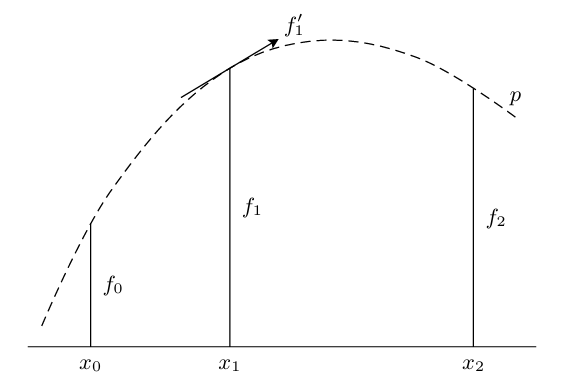
\includegraphics[width=0.75\textwidth]{images/hermite.png}
    \caption{Hermite 插值的例子}
    \label{fig::hermite_divided_difference}
\end{figure}

那么是否可以用 Lagrange 插值的思想来处理呢? 我们补充一个例子:

已知函数 $f(x)$ 在节点 $x_0, x_1, x_2$ 上的函数值 $y_0, y_1, y_2$ 和在 $x_1$ 处的导数值
$m_1$, 即                                                                           
$$
f(x_i) = y_i,\quad i = 0, 1, 2, \qquad f'(x_1) = m_1,
$$                                 
求一个次数不超过 $3$ 的多项式 $P(x)$, 使得                                            
$$
P(x_i) = y_i,\quad i = 0, 1, 2, \qquad P'(x_1) = m_1.
$$  

构造基函数. 设                                                                   
$$
P(x) = y_0 \varphi_0(x) + y_1 \varphi_1(x) + y_2 \varphi_2(x) + m_1 \psi(x)
$$                                 
其中假定 $\varphi_0(x), \varphi_1(x), \varphi_2(x), \psi(x)$ 都是3次多项式.
若它们分别满足下列条件:     
\begin{eqnarray}                                                                                    
&\varphi_0(x_0)=1, \quad &\varphi_0(x_1)=\varphi_0(x_2)=\varphi'_0(x_1)=0,\\             
&\varphi_1(x_1)=1,\quad &\varphi_1(x_0)=\varphi_1(x_2)=\varphi'_1(x_1)=0,\\             
&\varphi_2(x_2)=1,\quad &\varphi_2(x_0)=\varphi_2(x_1)=\varphi'_2(x_1)=0,\\             
&\psi'(x_1)=1,\quad &\psi(x_0)=\psi(x_1)=\psi(x_2)=0.                                   
\end{eqnarray}                                                                                      
则上述 $P(x)$ 即为所求.

于是                                                                                     
\begin{eqnarray*}                                                                                            
\varphi_0(x)&=&\frac{(x-x_1)^2(x-x_2)}{(x_0-x_1)^2(x_0-x_2)}\\                                       
\varphi_1(x)&=&(x-x_0)(x-x_2)\Big[\frac{(x_0+x_2-2x_1)}{x_1-x_0)^2(x_1-x_2)^2}(x-x_1)+\frac{1}{(x_1-\
x_0)(x_1-x_2)}\Big]\\                                                                               
\varphi_2(x)&=&\frac{(x-x_0)(x-x_1)^2}{(x_2-x_0)(x_2-x_1)^2}\\                                       
\psi(x)&=&\frac{(x-x_0)(x-x_1)(x-x_2)}{(x_1-x_0)(x_1-x_2)}                                           
\end{eqnarray*}                                                                                                  
得到$P(x)$.

当然, 在实际工作中, 要求得到节点处的精确导数是不太现实的要求. Hermite 插值
更多的用于一些公式的推导.




\bibliography{na.bib}
\bibliographystyle{plain}

\end{document}

